

\chapter{Technische Umsetzung} \label{implementation}

Die technische Umsetzung befasst sich mit der Implementation der aus dem Lösungsdesign gewonnenen Erkenntnisse. Dazu werden die vorgestellten Prinzipien des Software-Designs und der Algorithmus umgesetzt. Hierfür werden diese konkret in \gls{Typescript} programmiert und innerhalb der Applikationsstruktur platziert. Diese Struktur basiert zum einen auf dem bestehenden \gls{ikc-core} und zum anderen auf der vorgestellten Struktur innerhalb des \hyperref[architecture]{\textit{Kapitels der Architektur}}. Punktuell wird die Implementation zusätzlich durch die Nutzung von verschiedenen externen \gls{Bibliothek}[en] optimiert.

Die gezeigten Code-Ausschnitte werden bei Bedarf für dieses Dokument angepasst. Diese Änderungen dienen der Verständlichkeit im Kontext des Dokuments und beinhalten lediglich strukturelle, jedoch keine Änderungen an der Applikationslogik.



% -------------------------------


%    \begin{figure}[H]
%    \centering
%    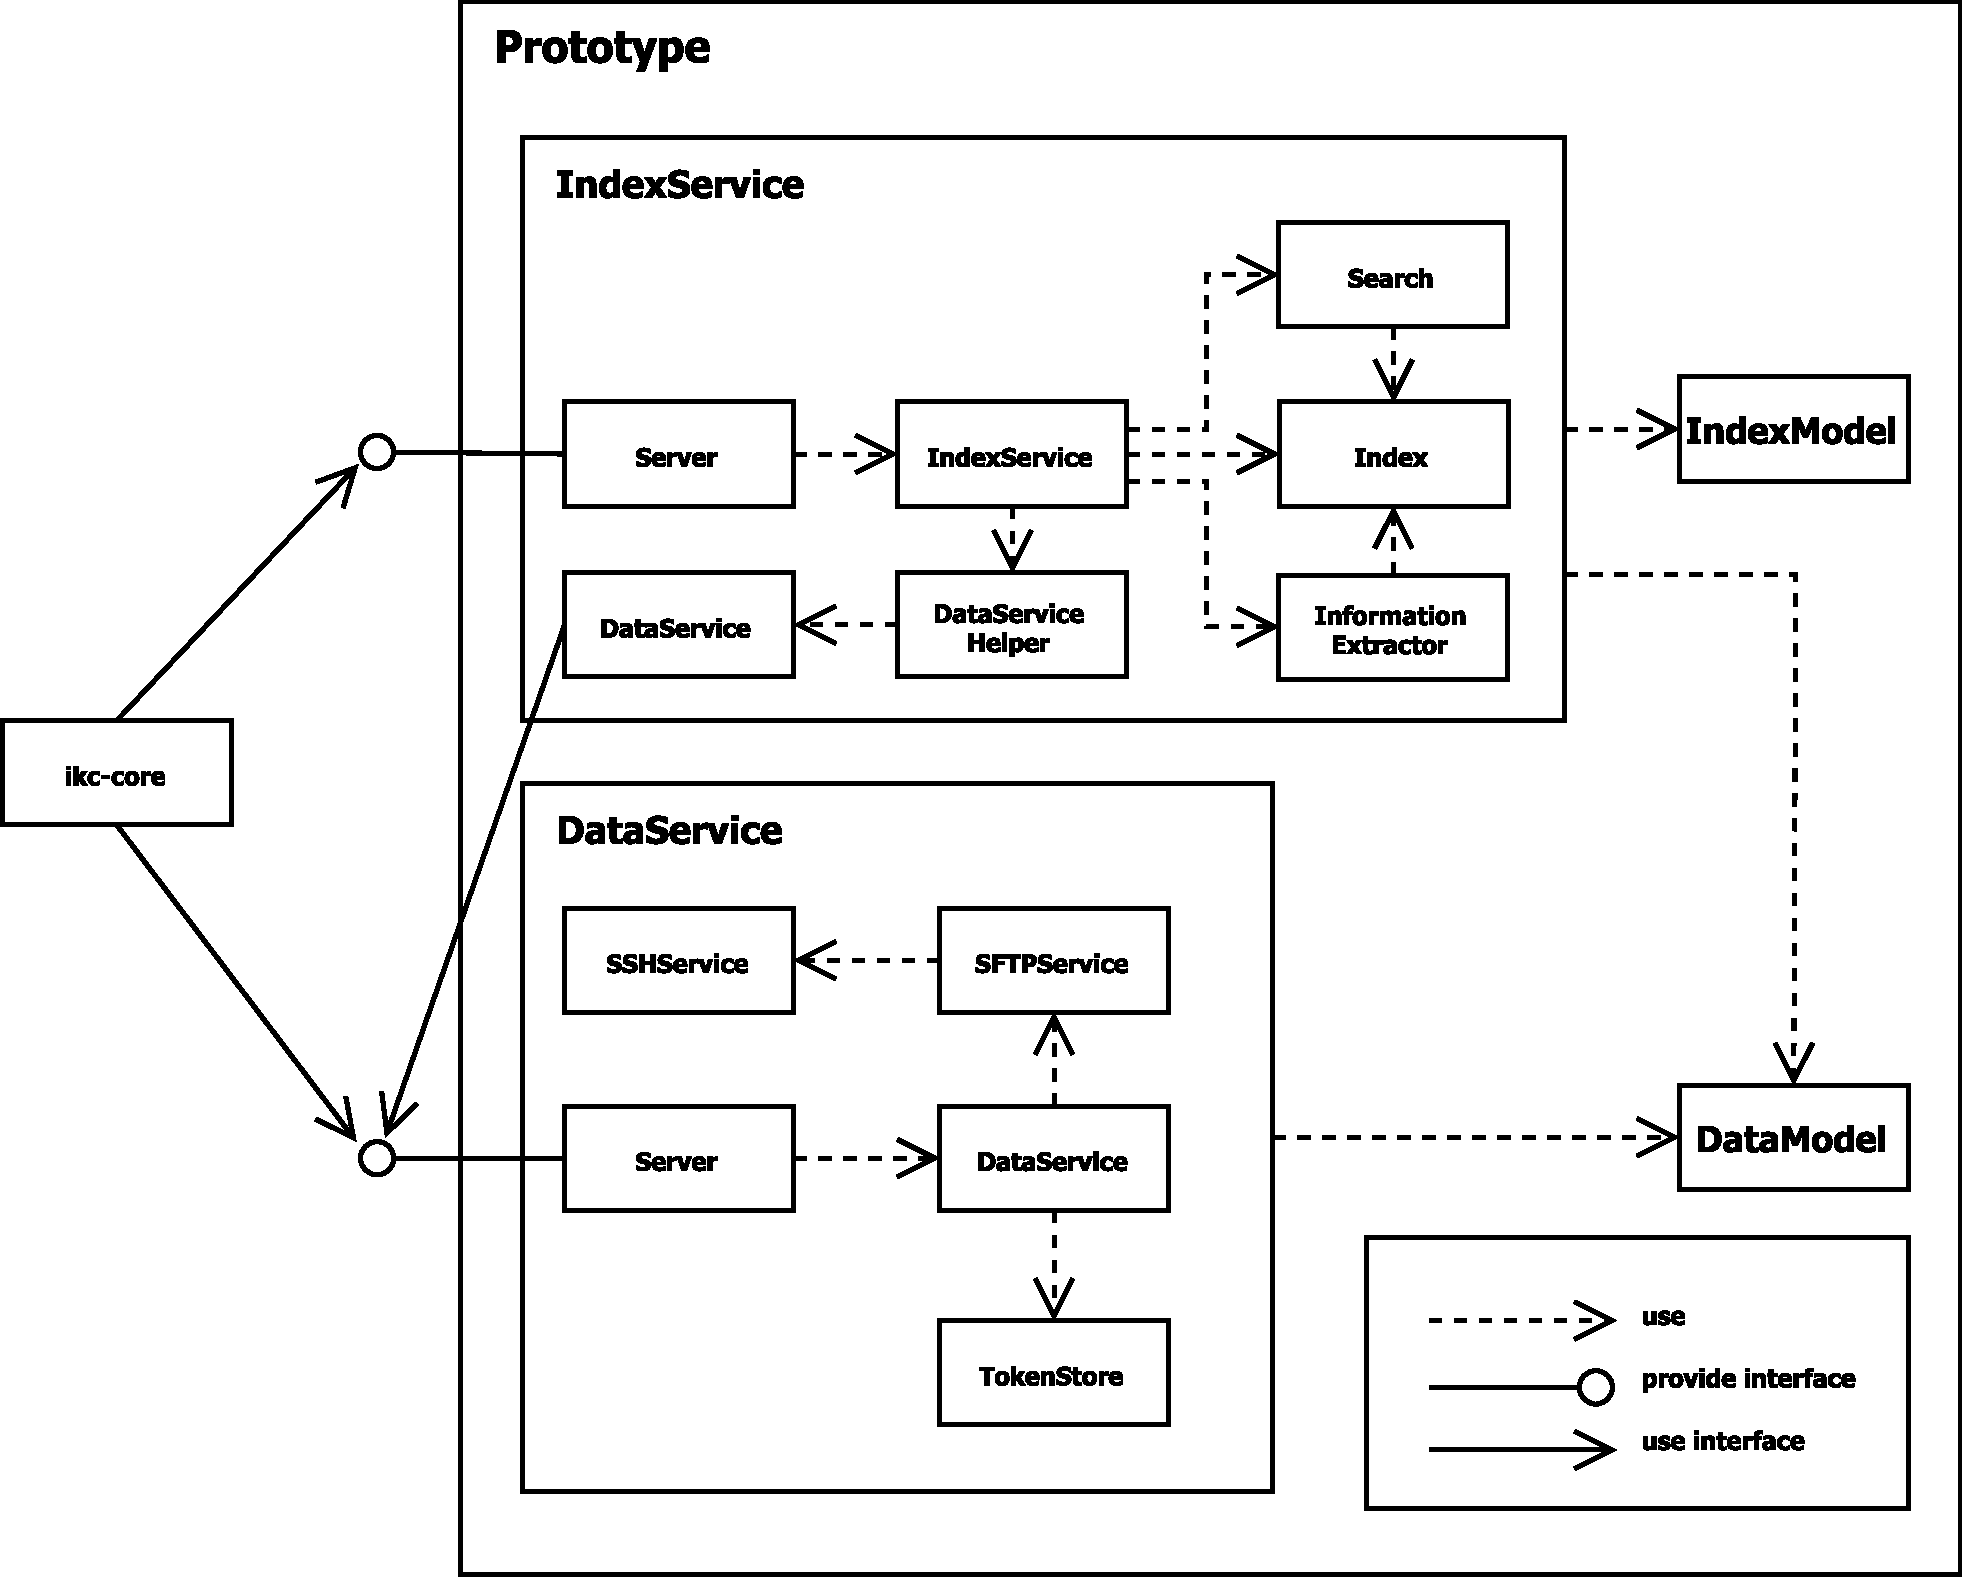
\includegraphics[width=1\textwidth]{PrototypeClassDiagram}
%    \caption{Prototype Klassendiagram}
%    \label{fig:prototypeClassDiagram}
%    \end{figure}

Der Kern der Software bildet der Algorithmus, dieser ist, neben der Suchfunktionalität und dem Aufbau der Indizes, ein Hauptbestandteil des \texttt{IndexService}. Der \autoref{indexservice} gewährt einen Überblick über die beteiligten Komponenten und deren ungefähre Funktionalität. Als Grund\-la\-ge benötigt der \texttt{In\-dex\-Ser\-vice} alle zu indexierenden Dateien im Volltext. Deren Quelle ist der \texttt{Data\-Ser\-vice}. Der \texttt{Index}- und der \texttt{Da\-ta\-Ser\-vi\-ce} bilden zusammen den eigentlichen Prototypen. Eine kurze Einführung folgt in den folgenden Abschnitten. Er\-wähn\-ens\-wer\-te weitere Themen in diesem Kapitel sind der Umgang mit Daten und die Kommunikation zwischen den verschiedenen Services. Wie in der Bausteinsicht auf \autoref{fig:bausteinsicht} zu erkennen ist, gibt es neben der Integration der Services auch eine Einbindung in die bestehende Benutzeroberfläche des \gls{ikc-core}.

% Folgend zunächst eine kurze Erklärung zu den einzelnen Klassen des \texttt{Index-} beziehungsweise \texttt{DataServices}.

\newpage

% ----------------------------------------------------------------

\section{IndexService}\label{indexservice}

% ----------------------------------------------------------------


Innerhalb des \texttt{IndexService} werden die primären Funktionen des Prototyps für die Schlüsselwort-Extraktion gekapselt. \autoref{fig:indexserviceClassDiagram} zeigt dabei, wie die wichtigsten Klassen miteinander kommunizieren. Anschliessend werden zentrale Abläufe genauer belichtet. 

    \begin{figure}[H]
    \centering
    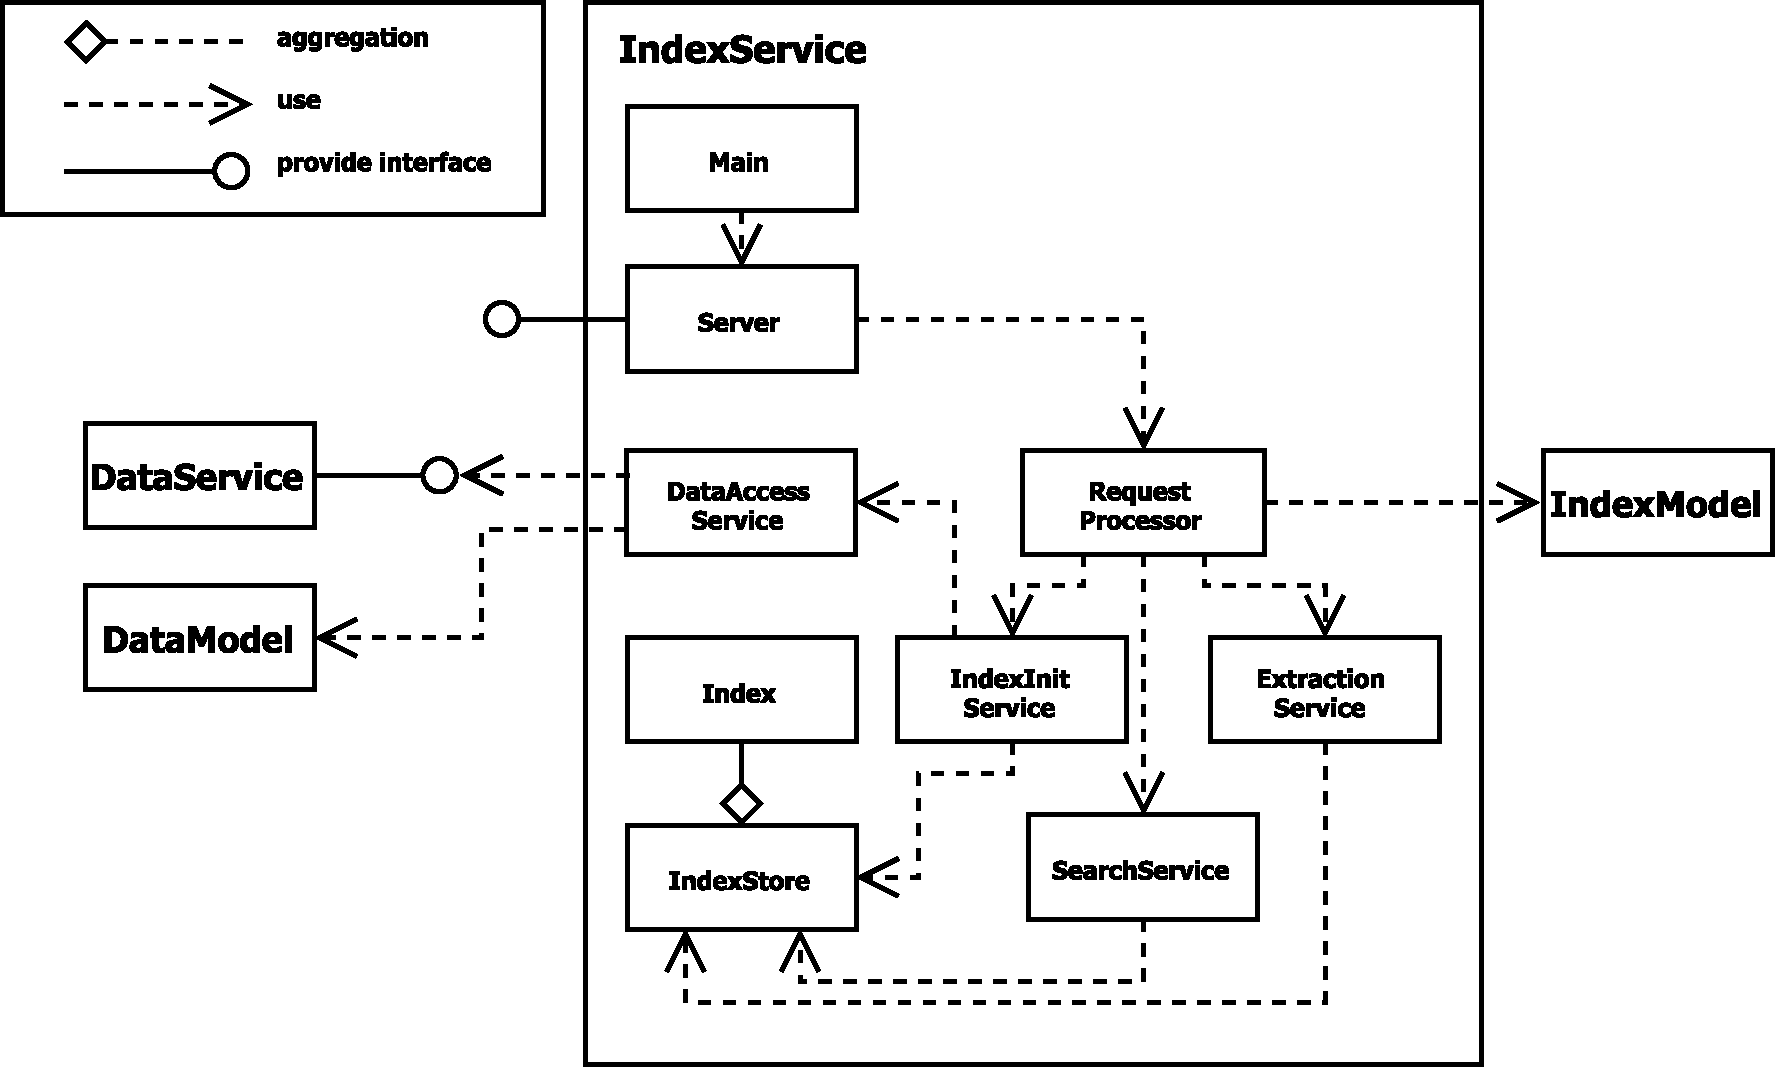
\includegraphics[width=1\textwidth]{IndexServiceClassDiagram}
    \caption{Klassendiagramm: IndexService}
    \label{fig:indexserviceClassDiagram}
    \end{figure}

\begin{itemize}
    \item \textbf{Main}: Die Klasse \texttt{Main} ist die zentrale Starter-Klasse des ganzen Services. Dazu initialisiert sie den Server. 
    \item \textbf{Server}: Hier werden Netzwerk-Anfragen entgegengenommen, und gegebenenfalls wird eine Antwort zu\-rück\-ge\-schi\-ckt.
    \item \textbf{Index}: Das Datenobjekt-\texttt{Index} hält alle Daten, welche für die Suche als auch für die Extraktion von \gls{Keyphrase}[s] und Dokumenten benötigt werden. Diese Klasse wird jedoch zur reinen Datenhaltung verwendet und beinhaltet keinerlei implementierte Logik. Sie beinhaltet den Volltext-Index und den Frequenz-Index. 
    \item \textbf{MessageManager}: Dies ist der Kern des \texttt{IndexService}: Anfragen werden basierend auf deren Typ für die Verarbeitung zu den drei Services \texttt{Search\-Ser\-vi\-ce}, \texttt{Ex\-trac\-tion\-Ser\-vi\-ce} und \texttt{In\-dex\-In\-it\-Ser\-vi\-ce} weitergeleitet.
    \item \textbf{IndexInitService}: Die Aufgabe, einen \texttt{Index} zu laden, hat der \texttt{IndexInitService}. Dazu kann er über den \texttt{DataAccessService} auf den \texttt{DataService} zugreifen, um die benötigten Daten abzufragen. Nach der Initialisierung wird der entsprechende \texttt{Index} innerhalb des \texttt{IndexStore} abgelegt.
    \item \textbf{SearchService}: Dieser Service ist verantwortlich für die Abarbeitung von Suchanfragen. Als Grundlage für die Resultate wird der Volltext-Index verwendet.  
    \item \textbf{ExtractionService}: Die Extraktion von \gls{Keyphrase}[s] oder Dokumenten wird durch den \texttt{ExtractionService} erledigt. 
    \item \textbf{DataAccessService}: Fungiert als Schnittstelle zum \texttt{DataService}.
    \item \textbf{IndexStore}: Beinhaltet alle geladenen \texttt{Index}-Objekte und stellt diese zur Verfügung. 
\end{itemize}


% ----------------------------------------------------------------

\subsection{Integration des Algorithmus}\label{impalgo}

% ----------------------------------------------------------------


Der vorgestellte Algorithmus wird innerhalb des \texttt{IndexService} in der Klasse \texttt{ExtractionHelper} implementiert. Sie stellt zwei Methoden, mit denen relevante \gls{Keyphrase}[s] (\texttt{getKeywordsForDocument}) oder relevante Dokumente (\texttt{getDocumentsForKeyword}) berechnet werden können, bereit. Da sie Funktionen bereit stellt, jedoch selbst keine Eigenschaften beispielsweise in Form von Variablen hält, muss ihr der benötigte Index mit der aufgerufenen Funktion zur Verfügung gestellt werden. 
Im Folgenden wird die Implementation der verschiedenen Schritte des Algorithmus genauer erläutert.

% ----------------------------------------------------------------

\subsubsection{Vorverarbeitung}

% ----------------------------------------------------------------

Im ersten Schritt geht es um die Vorverarbeitung des Texts. Dazu wird \gls{regex} verwendet, dadurch kann die Grösse des Codes erheblich reduziert werden im Vergleich zu einer Implementation ohne \gls{regex}. \autoref{preprocessing} zeigt die zwei nötigen Schritte:
\begin{itemize}
    \item Zuerst wird der Buchstabe, welcher auf einen Punkt, Fragezeichen, Ausrufezeichen oder Zeilenschaltung folgt, in die Kleinschreibung umgewandelt. Mithilfe des \gls{regex}-Ausdrucks werden diese erkannt und mittels einer anonymen Funktion transformiert.
    \item Anschliessend werden die einzelne Fragmente des Textes gebildet. Dazu wird ein \gls{regex}-Ausdruck verwendet, welcher eine Kollektion von Textfragmenten zurückgibt. Anders als beim vorherigen Schritt, wird eine Negation innerhalb des Ausdrucks verwendet. Dadurch werden nur Textfragmente ausgewählt, welche die entsprechenden Zeichen nicht enthalten. Somit enthält ein Fragment den Text zwischen einem Punkt und einem Komma oder innerhalb zweier Klammern. 
\end{itemize}

\begin{listing}[H]
\inputminted[
frame=lines,
framesep=2mm,
baselinestretch=1.2,
linenos,
breaklines=true
]{js}{sourcecode/IndexService/ExtractionHelper/processtext.ts}
\caption{Vorverarbeitung}
\label{preprocessing}
\end{listing}

% ----------------------------------------------------------------

\subsubsection{Text Zerlegung}

% ----------------------------------------------------------------

Die Textfragmente werden nun in die verschiedenen Wörter zerlegt. \autoref{listing:tokenization} zeigt die nötigen Schritte dazu:
\begin{itemize}
    \item Alle Fragmente werden bei einem Leerschlag aufgesplittet (Zeile 3).
    \item weiter werden \glqq's\grqq\, durch \glqq \: \grqq\, ersetzt (Zeile 6). Der apostrophierte Buchstabe S steht im Englischen (unter anderem) für den Genitiv. Da dies für die Auswertung (momentan) keine weitere Bedeutung hat, wird es ersatzlos gestrichen.
    \item Anschliessend werden unerwünschte Sonderzeichen zu Beginn oder am Ende eines Wortes mithilfe der Funktion \texttt{trimmer} der \gls{elasticlunr} Bibliothek entfernt (Zeile 5).
    \item Zum Schluss werden neu entstandere leere Wörter gefiltert, um diese nicht weiter zu verarbeiten (Zeile 9-11). 
\end{itemize}

\begin{listing}[H]
\inputminted[
frame=lines,
framesep=2mm,
baselinestretch=1.2,
linenos,
breaklines=true
]{js}{sourcecode/IndexService/ExtractionHelper/tokenization.ts}
\caption{Text Zerlegung}
\label{listing:tokenization}
\end{listing}

% ----------------------------------------------------------------

\subsubsection{Generierung möglicher Keyphrases}

% ----------------------------------------------------------------

Für die Generierung möglicher \gls{Keyphrase}[s] werden drei verschachtelte Schleifen verwendet. Die äusserste (Zeile 2) iteriert über die einzelnen Fragemente, die mittlere (Zeile 4) über die einzelnen Wörter innerhalb eines Textfragments und die innere (Zeile 12) über die Länge der \gls{N-Gramm}[e] von eins bis \texttt{n}.
\autoref{generatekeywords} zeigt den genaueren Ablauf und in \autoref{fig:exampleloop} (Zeile 2 $\rightarrow$ \textit{\textbf{rot}}, Zeile 4 $\rightarrow$ \textit{\textbf{grün}}, Zeile 12 $\rightarrow$ \textit{\textbf{blau}}) ist ein genaueres Beispiel der drei Schleifen ersichtlich :
\begin{itemize}
     \item Falls ein \gls{N-Gramm} länger als die verbliebene Anzahl Wörter innerhalb des Fragments ist, muss die maximale Länge reduziert werden. Wenn zum Beispiel noch zwei Wörter übrig bleiben, können nur noch \textit{2-Gramme} und \textit{1-Gramme} gebildet werden. Die Länge muss zusätzlich auf \texttt{length = 2} reduziert werden (Zeile 6-9).
     \item Um die \gls{N-Gramm}[e] zu generieren, wird nun eine Liste von Wört\-ern aus dem Fragment ausgelesen. Dies geschieht mithilfe der Methode \texttt{slice}. Anschliessend werden diese mit \texttt{join} zu einer \gls{Keyphrase} zusammengeführt. Beide Methoden sind Teil der standardmässigen \texttt{Array}-Klasse von Typescript (Zeile 13-14).
     \item Schlussendlich werden nun die generierten \gls{N-Gramm}[e] (\gls{Keyword}[s]) in einer Map zusammen mit ihrer Häufigkeit abgelegt.
\end{itemize}

\begin{listing}[H]
\inputminted[
frame=lines,
framesep=2mm,
baselinestretch=1.2,
linenos,
breaklines=true
]{js}{sourcecode/IndexService/ExtractionHelper/generate-keywords.ts}
\caption{Keywords Generierung}
\label{generatekeywords}
\end{listing}

\begin{figure}[H]
\centering
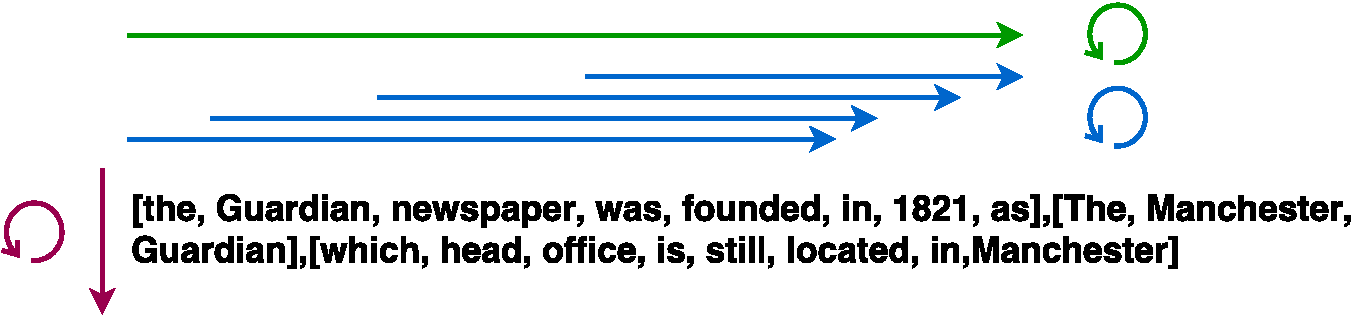
\includegraphics[width=1\textwidth]{exampleloop}
\caption{Beispiel Schlaufe}
\label{fig:exampleloop}
\end{figure}


% ----------------------------------------------------------------

\subsubsection{Filter mittels POS-Tagger}

% ----------------------------------------------------------------

Bevor die Relevanz der \gls{Keyphrase}[s] berechnet werden kann, werden sie ein weiteres Mal reduziert. Dies passiert mithilfe eines Filters basierend auf dem POS-Tagger. Dieser Filter wird direkt auf jedes einzelne mögliche \gls{Keyphrase} angewendet, innerhalb der äussersten Schleife in \autoref{generatekeywords} (Zeile Dazu zeigt \autoref{filter} die nötigen Schritte auf.
\begin{itemize}
    \item Für jede mögliche \gls{Keyphrase} werden die Wortarten der einzelnen Wörter berechnet. Dies wird mittels der Methode \texttt{tag} aus der externen Bibliothek \textit{pos-js}\footnote{\url{https://github.com/dariusk/pos-js}} durchgeführt. Als Resultat wird ein \texttt{Array} zurückgegeben, welches für jedes Wort wiederum ein \texttt{Array} enthält. Dieses enthält einen Eintrag mit dem Wort und der zugehörigen Wortart. Neben der Wortart wird zum Beispiel auch die Zeit eines Verbs oder der Numerus eines Nomens erkannt. Innerhalb der Dokumentation der Bibliothek ist eine Liste mit allen möglichen Resultaten angefügt. Anschliessend wird die jeweilige \gls{Keyphrase} mithilfe der drei Methoden \texttt{properNGramPos}, \texttt{properNGramStart} und \texttt{properNGramEnd} auf ihre Gültigkeit geprüft. Dies geschieht aufgrund der definierten Vorgaben (\autoref{algo}) (Zeile 2). 
    \item Als erstes wird überprüft, ob das \gls{Keyword} ein Nomen oder ein fremdes Wort enthält (Zeile 4-13).
    \item Weiter muss die \gls{Keyphrase} entweder mit einem Nomen, einem Adjektiv, einem fremden Wort oder in Grosschreibung starten (Zeile 15-24).
    \item Schlussendlich muss eine gültiges \gls{Keyphrase} auch mit einem Nomen, einem Adjektiv oder einem fremden Wort enden (Zeile 26-32).
\end{itemize}

\begin{listing}[H]
\inputminted[
frame=lines,
framesep=2mm,
baselinestretch=1.2,
linenos,
breaklines=true
]{js}{sourcecode/IndexService/ExtractionHelper/filter.ts}
\caption{Filter}
\label{filter}
\end{listing}


% ----------------------------------------------------------------

\subsubsection{Berechnung der Relevanz}

% ----------------------------------------------------------------

Der wichtigste Schritt für die Bewertung der einzelnen \gls{Keyphrase}[s] ist der berechnete Wert, dieser folgt aus der entsprechenden Formel (\autoref{algo}). Die verschiedenen Schritte werden im \autoref{calc} genauer erläutert:
\begin{itemize}
    \item Als erstes muss die Länge des Korpus \texttt{indexLength} berechnet werden. Diese kann direkt aus dem Volltext-Index abgefragt werden. Dazu wird die Länge des \texttt{documentStore} berechnet. Anschliessend wird die Anzahl Dokumente \texttt{keywordDocFreq} mit diesem \gls{Keyphrase} berechnet. Dieser Wert kann direkt aus dem Frequenz-Index gelesen werden. Zum Schluss muss noch die Anzahl Wörter innerhalb des Dokuments der \gls{Keyphrase} berechnet werden (Zeile 2-6). 
    \item Basierend auf der Anzahl Dokumente (\texttt{indexLength}) und der Anzahl Dokumente mit dem \gls{Keyword} (texttt{keywordDocFreq}) wird als nächstes nun der \textit{IDF}-Wert (\texttt{keywordIdf}) berechnet (Zeile 8). \item Den \textit{TF}-Wert (\texttt{keywordTf}) wird bereits mit der \gls{Keyphrase} mitgeliefert (Zeile 10).
    \item Anhand der Dokumentenlänge wird nun eine entsprechende Normierung (\texttt{lengthNorm}) für den \gls{Score} berechnet (Zeile 12).
    \item Schlussendlich werden die verschiedenen Werte untereinander multipliziert, um den entsprechenden \gls{Score} zu erhalten (Zeile 14).
\end{itemize}

\begin{listing}[H]
\inputminted[
frame=lines,
framesep=2mm,
baselinestretch=1.2,
linenos,
breaklines=true
]{js}{sourcecode/IndexService/ExtractionHelper/calc.ts}
\caption{Berechnung Relevanz}
\label{calc}
\end{listing}

% ----------------------------------------------------------------

\subsubsection{Auswahl}

% ----------------------------------------------------------------

Nach der Berechnung des \gls{Score}[s] wird die Liste mit \gls{Keyphrase}[s] absteigend sortiert und mit Hilfe eines Schwellwertes begrenzt.

\subsubsection{Dokument Extraktion}
Die entsprechenden Dokumente, welche eine bestimmte \gls{Keyphrase} beinhalten, können direkt aus dem Frequenz-Index ausgelesen werden. Dies geschieht durch die folgenden Schritte (\autoref{doc-extraction}):
\begin{itemize}
    \item Mithilfe der \gls{Keyphrase} kann innerhalb des Frequenz-Index eine Liste mit passenden Dokumente abgefragt werden (Zeile 2).
    \item Anschliessend werden die gleichen Berechnungen wie in \autoref{calc} durchgeführt, um die Relevanz der einzelnen Dokumente für die \gls{Keyphrase} zu berechnen. Die Anzahl der Vorkommnisse innerhalb des einzelnen Dokuments kommt zusammen mit dem Dokument aus dem Frequenz-Index (Zeile 3-10).
\end{itemize}

\begin{listing}[H]
\inputminted[
frame=lines,
framesep=2mm,
baselinestretch=1.2,
linenos,
breaklines=true
]{js}{sourcecode/IndexService/ExtractionHelper/doc-extraciton.ts}
\caption{Dokument-Extraktion}
\label{doc-extraction}
\end{listing}

% ----------------------------------------------------------------

\subsection{Index-Aufbau}\label{indexstructure}

% ----------------------------------------------------------------

Innerhalb der \texttt{Index}-Klassen wird der Volltext-Index als auch der Frequenz-Index gehalten. \autoref{fig:indexclassdiagramm} zeigt den Aufbau der Klasse:
\begin{itemize}
  \item Der Volltext-Index ist innerhalb des Objekts \texttt{searchIndex} gespeichert. Dazu wird die externe Bibliothek \gls{elasticlunr} verwendet. Sie wurde aus den folgenden beiden Gründen ausgewählt:
  \begin{enumerate}
       \item Sie basiert auf dem Volltext-Index \gls{lunr}, welcher bereits innerhalb des \gls{ikc-core} verwendet wird. Da trotz der Weiterentwicklung die grundlegende Handhabung gleich geblieben ist, kann bestehender Code wiederverwendet werden.
       \item \gls{elasticlunr} basiert auf einem äusserst schlanken Index und erreicht so eine kurze Abfragezeit. Gerade die Grösse ist entscheidend, um den Index schnell übertragen zu können.
       \item Als Opensource-Projekt können einzelne Anpassungen direkt gemacht und so an die individuellen Bedürfnisse angepasst werden. Weiter gibt es eine aktive Community, das Projekt wird laufend gewartet und weiterentwickelt.
  \end{enumerate}
  \item Innerhalb des Objekts \texttt{freqIndex} wird der Frequenz-Index gehalten. \autoref{freqindex} zeigt den Aufbau des selbst implementierten Index. Dieser besteht grundsätzlich aus einer Liste aller \gls{Keyphrase}[s] aus allen Dokumenten. Zu jeder \gls{Keyphrase} wird nun die Anzahl (\texttt{f}) Dokumente, welche diese \gls{Keyphrase} enthalten und die entsprechenden Dokumente \texttt{docs} gespeichert. Weiter wird zu jedem Dokument die Häufigkeit der \gls{Keyphrase} innerhalb des Dokuments und eine eindeutige Identifikation des Dokuments gespeichert. Der Frequenz-Index wird benötigt, um die Berechnung der relevanten \gls{Keyphrase}[s] zu beschleunigen. Insbesondere die Berechnung der Anzahl der Dokumente, welche eine bestimmte \gls{Keyphrase} enthalten, wird mit zunehmender Grösse des Index sehr zeitintensiv. 
  \item Der \texttt{timestamp} wird zur Versionierung des \texttt{Index} verwendet.
\end{itemize}


    \begin{figure}[H]
    \centering
    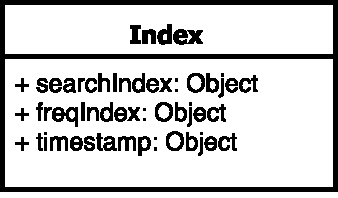
\includegraphics[width=0.3\textwidth]{IndexClassDiagramm}
    \caption{Klassendiagramm: Index}
    \label{fig:indexclassdiagramm}
    \end{figure}
    
\begin{listing}[H]
\inputminted[
frame=lines,
framesep=2mm,
baselinestretch=1.2,
linenos,
breaklines=true
]{js}{sourcecode/IndexService/freqIndex.ts}
\caption{Frequenz-Index}
\label{freqindex}
\end{listing}

% ----------------------------------------------------------------
    
\subsection{Index-Initialisierung}

% ----------------------------------------------------------------

Die Berechnung des Index ist eine der prozessorintensiven Aufgaben, sie ist Zeit- und Ressourcen-intensiv. Dies insbesondere aufgrund der vielen Lese-Zugriffe. Darum wird der Index, wann immer möglich zwischengespeichert, sodass eine erneute Berechnung erspart bleibt. Sie bildet die Grundlage für die zentralen Funktionen (\gls{Keyword}-Ex\-trak\-tion und Suche) des Prototyps. Um den Index zu initialisieren werden drei verschiedenen Szenarien unterschieden, der Ausgang diese Szenarien ist dabei immer der \gls{ikc-core}:
\begin{itemize}
    \item \textbf{Index berechnen}: Es wurde noch kein Index berechnet, daher muss er von Grund auf neu berechnet werden.
    \item \textbf{Index einlesen}: Der Index wurde bereits berechnet, jedoch noch nicht eingelesenen und ist darum noch nicht bereit für die Verwendung. Dazu müssen die nötigen Daten abgefragt und eingelesen werden.
    \item \textbf{Index bereit}: Der \texttt{IndexService} hat den Index bereits eingelesen und er ist bereit für die Verwendung.
\end{itemize}

Folgend werden die verschiedenen Szenarien genauer erklärt.

% ----------------------------------------------------------------

\subsubsection{Index-Berechnung}

% ----------------------------------------------------------------

\autoref{fig:seqindexalreadybuilt} zeigt den aufwändigen Ablauf der Index-Berechnung. 
\begin{itemize}
    \item \texttt{requestIndex}: Der \gls{ikc-core} möchte Zugriff auf den Index. Dafür tätigt er eine Anfrage beim \texttt{IndexService}. Da der Index weder geladen, noch berechnet wurde, muss dieser neu berechnet werden.
    \item \texttt{dataRequest}: Dafür müssen zunächst alle Dokumente eingelesen werden. Dafür muss eine Anfrage an den \texttt{DataService} gemacht werden.
    \item \texttt{dataResponse}: Diese wird mit den geforderten Daten beantwortet.
    \item \texttt{parseData}: Die Daten werden geparst, damit sie weiterverarbeitet werden können.
    \item \texttt{buildIndex}: Nun wird jedes einzelne Dokument dem Index hinzugefügt. \autoref{calcindex} zeigt die verschiedenen Schritte, welche dabei ausgeführt werden:
    \begin{enumerate}
        \item Das entsprechende Dokument wird dem \texttt{searchIndex} mithilfe der Methode \texttt{addDoc} hinzugefügt. Pro Dokument werden die drei Felder \texttt{body} (Inhalt), \texttt{title} (Title) und \texttt{length} (Anzahl Wörter) verwendet. Neben dem Dokument-Objekt muss \texttt{addDoc} auch noch eine eindeutige Identifikation mitgegeben werden, hier die \texttt{doc.id}. Die Anzahl der Wörter wird später für die Berechnung der relevanten Dokumente für eine bestimmte \gls{Keyphrase} verwendet (Zeile 2-6). 
        \item Nun werden für das entsprechende Dokument die mög\-lich\-en \gls{Keyphrase}[s] extrahiert. Dazu werden gleiche Berechnungen verwendet, wie in \autoref{listing:tokenization}, \autoref{generatekeywords} und \autoref{filter} (Zeile 8).
        \item Nun werden zum Abschluss die \gls{Keyphrase}[s] nach dem beschriebenen Schema (\autoref{indexstructure} dem Frequenz-Index hinzugefügt (Zeile 10-21).
    \end{enumerate}
    \item \texttt{saveIndex}: Sobald der Index berechnet wurde, wird er im \texttt{In\-dex\-Store} gespeichert.
    \item \texttt{indexReady}: Dem \gls{ikc-core} wird gemeldet, dass der Index bereit ist.
\end{itemize}

    \begin{figure}[H]
    \centering
    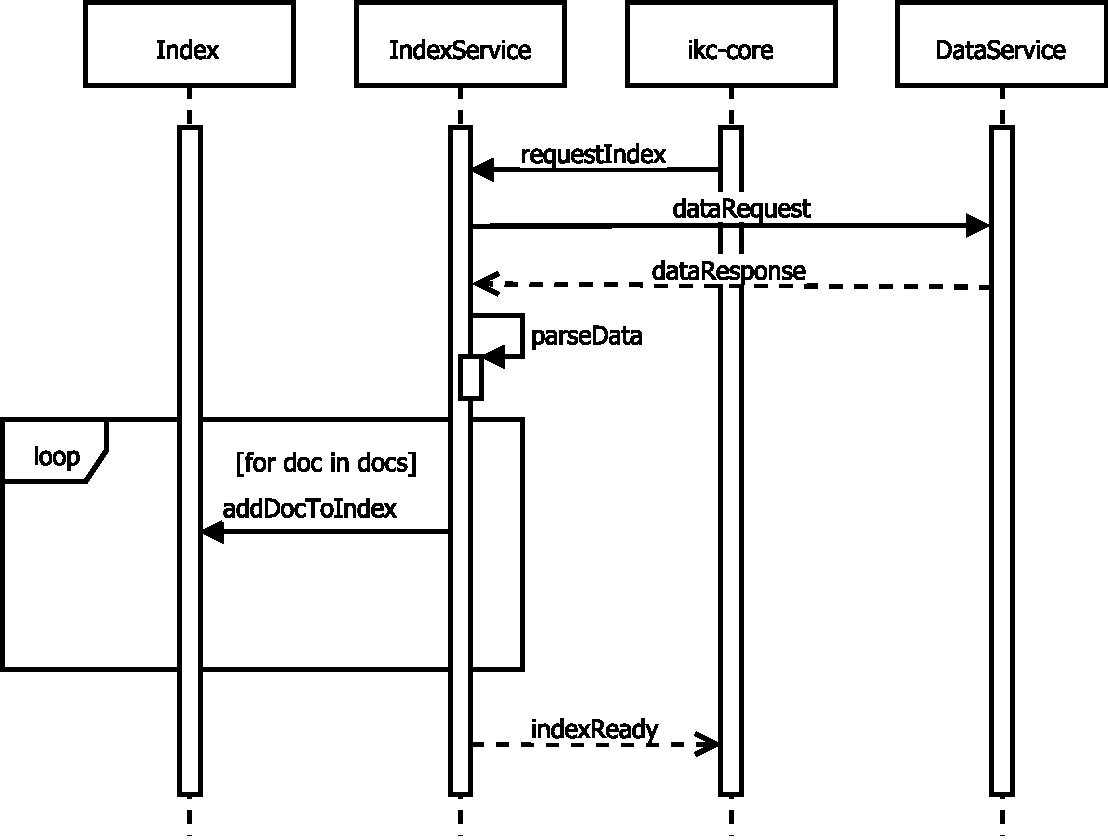
\includegraphics[width=1\textwidth]{SeqIndexLoad}
    \caption{Ablauf: Index-Berechnung}
    \label{fig:seqindexload}
    \end{figure}


\begin{listing}[H]
\inputminted[
frame=lines,
framesep=2mm,
baselinestretch=1.2,
linenos,
breaklines=true
]{js}{sourcecode/IndexService/calcIndex.ts}
\caption{Berechnung: Index}
\label{calcindex}
\end{listing}

    
% ----------------------------------------------------------------
    
\subsection{Index speichern}

% ----------------------------------------------------------------

Durch die Speicherung des Index werden die berechneten Daten gesichert und so eine aufwändige Neuberechnung verhindert. \autoref{fig:seqwriteindex} zeigt die einzelnen Schritte auf:
\begin{itemize}
    \item Das Speichern des Index wird durch den \gls{ikc-core} ausgelöst.
    \item Anschliessend wird der Index präpariert, um diesen Persistieren zu können. Dazu sind die in \autoref{writeindex} beschriebenen Schritte notwendig:
    \begin{enumerate}
        \item Als erstes muss die \texttt{toJSON} Methode des \gls{elasticlunr} Objekts aufgerufen werden. Dadurch werden intern Funktionen für die Serialisierung vorbereitet (Zeile 2).
        \item Mit Hilfe der Bibliotheken \gls{msgpack} und \gls{lz4} werden die beiden Indizes zuerst serialisiert und anschliessend komprimiert (Zeile 4-5).
        \item Zum Schluss werden beide resultierenden Buffer in einem einzelnen Buffer zusammengefasst (Zeile 7-11). Dabei werden diese mittels \gls{msgpack} erneut serialisiert.
    \end{enumerate}
    \item Zum Speichern wird der präparierte Index schlussendlich an den \texttt{DataService} gesendet. 
\end{itemize}

    \begin{figure}[H]
    \centering
    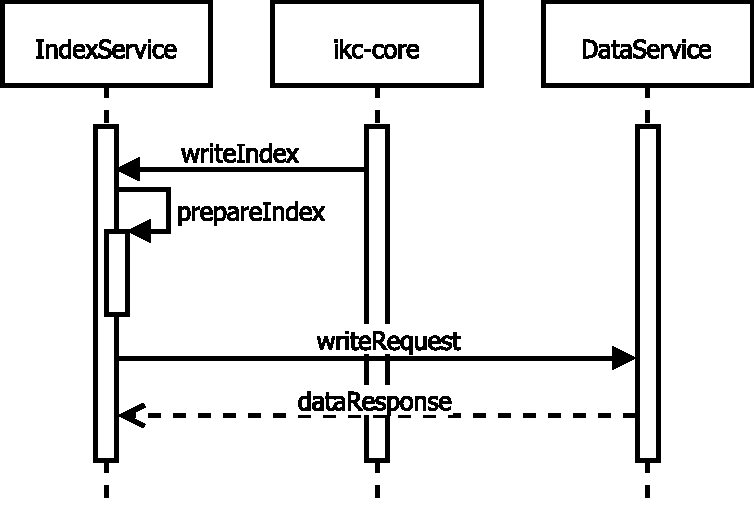
\includegraphics[width=0.5\textwidth]{SeqWriteIndex}
    \caption{Ablauf: Index speichern}
    \label{fig:seqwriteindex}
    \end{figure}

\begin{listing}[H]
\inputminted[
frame=lines,
framesep=2mm,
baselinestretch=1.2,
linenos,
breaklines=true
]{js}{sourcecode/IndexService/writeIndex.ts}
\caption{Index Speichern}
\label{writeindex}
\end{listing}
    

% ----------------------------------------------------------------
    
\subsubsection{Index einlesen}

% ----------------------------------------------------------------


Falls ein Index bereits berechnet und persistiert wurde, muss er lediglich eingelesen werden. Dieser Ablauf wird in der \autoref{fig:seqindexalreadybuilt} erläutert. 
\begin{itemize}
    \item \texttt{requestIndex}: Der \gls{ikc-core} möchte Zugriff auf den Index. Dafür tätigt er eine Anfrage beim \texttt{IndexService}. Der \texttt{IndexService} hat den Index nicht geladen, er startet also die Berechnung.
    \item \texttt{dataRequest}: Nun muss das serialisierte Index-Objekt geladen werden. Dafür muss eine Anfrage an den \texttt{DataService} gemacht werden.
    \item \texttt{dataResponse}: Diese wird mit den geforderten Daten beantwortet.
    \item Die Daten werden eingelesen (\texttt{parseData}) und anschliessend verarbeitet (\texttt{loadIndex}). Die verschiedenen Schritte werden in \autoref{parseindex} detailliert erläutert.
    \begin{enumerate}
        \item Die empfangenen Daten (\texttt{body}) müssen mithilfe der externen Bibliothek \gls{msgpack}\footnote{\url{http://msgpack.org}} decodiert werden. Daraus folgen die beiden \gls{Buffer} für den Volltext- und Frequenz-Index.
        \item Nun werden die beiden \gls{Buffer} zuerst mit Hilfe der Bibliothek \gls{lz4} dekomprimiert und anschliessend durch \gls{msgpack} erneut decodiert. Die Decodierung generiert aus dem Buffer ein Objekt (Zeile 3-4).
        \item Nun werden die decodierten Objekte dem \texttt{Index} zugwiesen. Der Volltext-Index muss zuerst noch durch die \texttt{load}-Methode des \gls{elasticlunr} eingelesen werden (Zeile 6-7).
    \end{enumerate}
    \item \texttt{indexReady}: Dem \gls{ikc-core} wird gemeldet, dass der Index bereit ist.
\end{itemize}

    \begin{figure}[H]
    \centering
    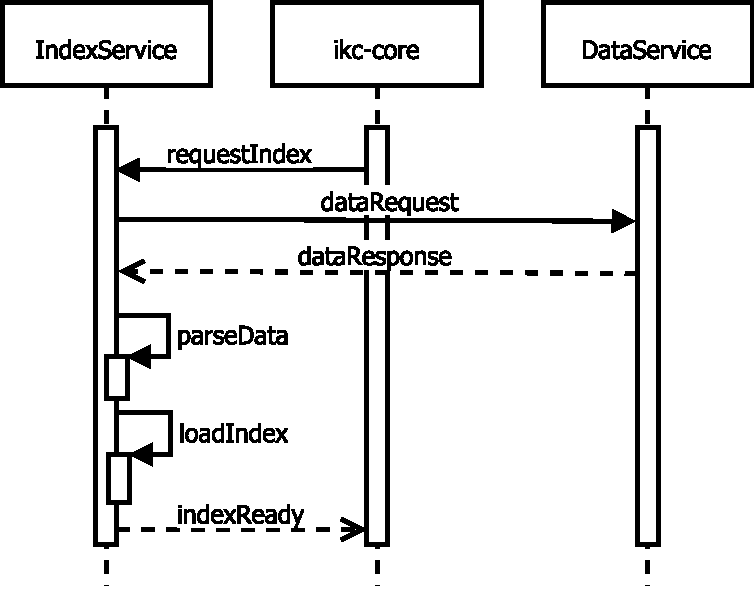
\includegraphics[width=1\textwidth]{SeqIndexLoadAlreadyBuilt}
    \caption{Ablauf: Index-Berechnung}
    \label{fig:seqindexalreadybuilt}
    \end{figure}
    
\begin{listing}[H]
\inputminted[
frame=lines,
framesep=2mm,
baselinestretch=1.2,
linenos,
breaklines=true
]{js}{sourcecode/IndexService/parseIndex.ts}
\caption{Laden: Index-Objekt}
\label{parseindex}
\end{listing}
    
% ----------------------------------------------------------------
    
\subsubsection{Index bereit}

% ----------------------------------------------------------------


Die \autoref{fig:seqindexloadalreadydone} hingegen zeigt den Ablauf, falls der Index bereits im \texttt{IndexService} geladen ist.

\begin{itemize}
    \item \texttt{requestIndex}: Der \gls{ikc-core} benötigt den Index. Dafür fragt er den \texttt{IndexService} an. Dieser hält den Index bereits im Ar\-beits\-spei\-cher.
    \item \texttt{indexReady}: Somit kann er diesen direkt zurückliefern.
\end{itemize}
    
    \begin{figure}[H]
    \centering
    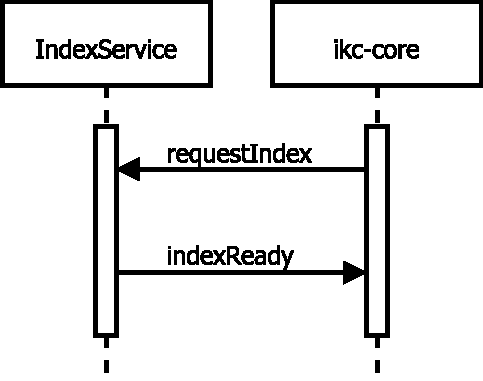
\includegraphics[width=0.5\textwidth]{SeqIndexLoadAlreadyDone}
    \caption{Ablauf: Index-Zugriff}
    \label{fig:seqindexloadalreadydone}
    \end{figure}

 
% ----------------------------------------------------------------
     
\subsection{Keyword-Extraktion}

% ----------------------------------------------------------------


Die \gls{Keyword}-Extraktion ist eine der wichtigsten Funktionen des Prototypen. Dabei werden die vorgestellten Abläufe und auch die Code-Ausschnitte aus dem \autoref{impalgo} verwendet. In der nachfolgenden \autoref{fig:seqkeywordextraction} wird der Ablauf genauer erläutert:
\begin{itemize}
    \item Initiiert wird die Extraktion von \gls{Keyphrase}[s] durch die \texttt{Key\-word\-Re\-qu\-est}-Nachricht, welche der \gls{ikc-core} an den \texttt{IndexService} sendet. Anschliessend wir das entsprechende Dokument vom \texttt{Da\-ta\-Ser\-vi\-ce} bezogen und für die Verarbeitung aufbereitet. 
    \item Innerhalb des \texttt{IndexService} werden die relevanten \gls{Keyphrase}[s] durch den \texttt{ExtractionService} berechnet und zurückgegeben.
    \item Anschliessend werden die \gls{Keyphrase}[s] innerhalb einer \texttt{Key\-word\-Re\-spon\-se} Nachricht an den \gls{ikc-core} gesendet.
\end{itemize}

    \begin{figure}[H]
    \centering
    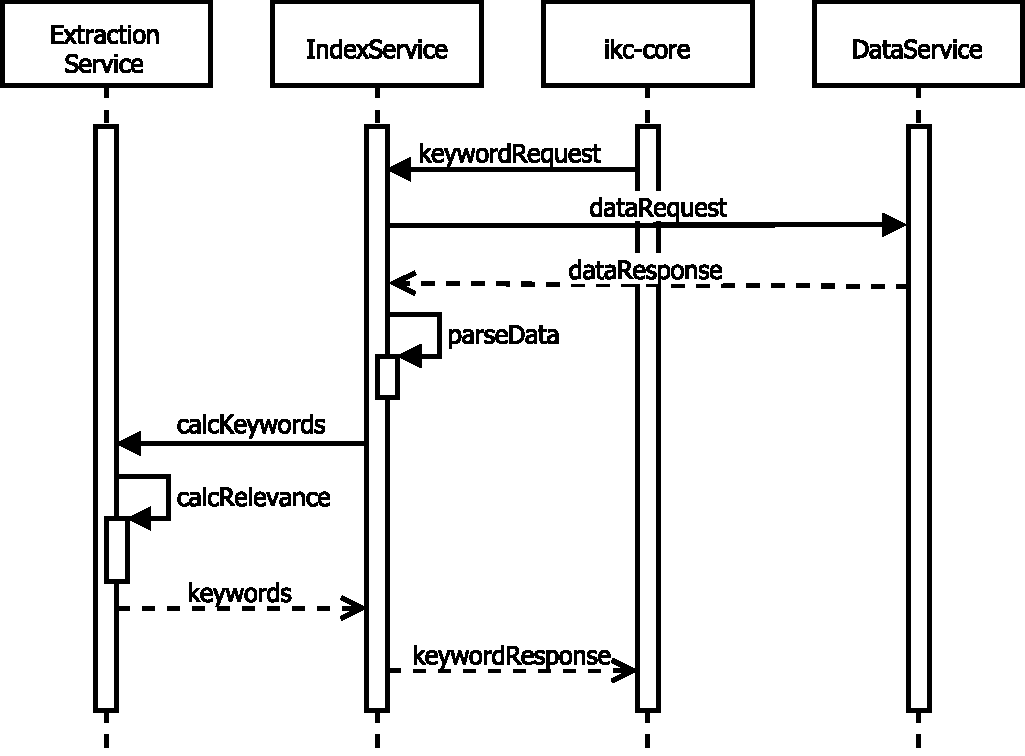
\includegraphics[width=1\textwidth]{SeqGetKeyword}
    \caption{Ablauf: \gls{Keyword}-Extraktion}
    \label{fig:seqkeywordextraction}
    \end{figure}

% ----------------------------------------------------------------

\subsection{Dokument-Extraktion}

% ----------------------------------------------------------------


Neben der Extraktion von \gls{Keyphrase}[s] sollen pro \gls{Keyphrase} auch passende Dokumente extrahiert werden. Dieser Ablauf ist in der \autoref{fig:seqdocument} ersichtlich.

    \begin{figure}[H]
    \centering
    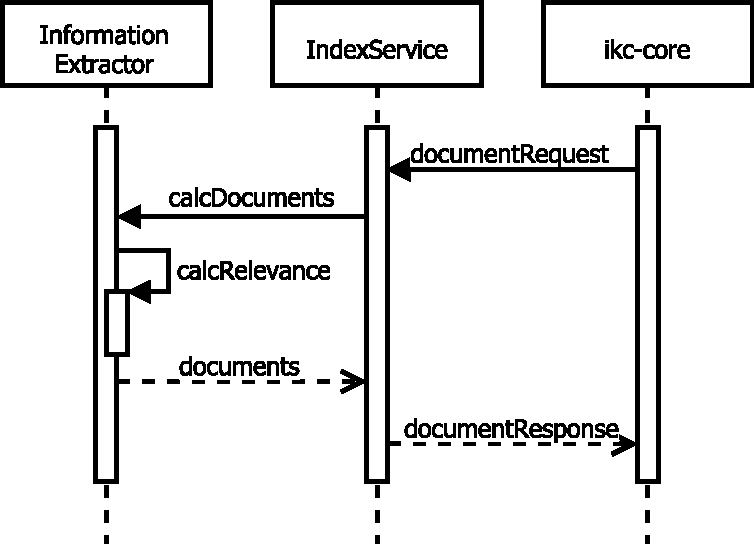
\includegraphics[width=0.8\textwidth]{SeqDocument}
    \caption{Ablauf: Dokument-Extraktion}
    \label{fig:seqdocument}
    \end{figure}

\begin{itemize}
    \item Der \gls{ikc-core} fordert durch eine \texttt{DocumentRequest} eine Liste von Dokumenten für eine \gls{Keyphrase} an. 
    \item Anschliessend extrahiert der \texttt{InformationExtractor} eine Liste von passenden Dokumenten und bewertet ihre Relevanz. 
    \item Innerhalb einer \texttt{DocumentResponse}-Nachricht wird die resultierende Liste an den \gls{ikc-core} gesendet und die Anfrage somit beendet.
\end{itemize}

% ----------------------------------------------------------------

\subsection{Suche}

% ----------------------------------------------------------------

Eine Volltextsuche macht macht die ganzen Dantenquellen durchsuchbar. Mit Hilfe der folgenden \autoref{fig:seqsearch} wird der Ablauf der Suche aufgezeigt:
\begin{itemize}
    \item Innerhalb des \gls{ikc-core} wird eine Suchanfrage abgesetzt. Diese erreicht den \texttt{IndexService} eingebettet in einer \texttt{SearchRequest}-Nachricht. 
    \item Intern arbeitet der \texttt{SearchService} die Suche ab und liefert die entsprechenden Resultate. \autoref{search} zeigt den Ablauf innerhalb des \texttt{SearchService}:
    \begin{enumerate}
        \item Um eine Suche durchführen zu können, muss zuerst eine Konfiguration erstellt werden. Diese folgt der API Dokumentation von \gls{elasticlunr}. So wäre es möglich, verschiedene Felder unterschiedlich zu gewichten. Auf diese Option wird jedoch verzichtet, lediglich die Option \texttt{bool} wird auf \texttt{AND} gesetzt. Damit müssen resultierende Dokumente alle Wörter der Suchanfrage enthalten. Eine andere Option wäre \texttt{OR}, damit würden Dokumente resultieren, die mindestens ein Wort der Suchanfrage enthalten (Zeile 2).
        \item Nun wird die eigentliche Suchanfrage ausgeführt, dazu wird die Methode \texttt{search} verwendet. Ihr wird der Suchterm (\texttt{term}) und die Konfiguration mitgegeben. Als Resultat wird eine Liste von Dokumentation-Ids zusammen mit dem \gls{Score} absteigend sortiert zurückgegeben (Zeile 4).
        \item Durch die hohe Anzahl der zu erwartenden Dokumente kann die Anzahl der Suchresultate sehr schnell gross werden. Um das Resultat einschränken zu können, werden nur die 100 besten Resultate angezeigt. Dies geschieht mithilfe der \texttt{slice}-Methode der \texttt{Array}-Klasse. Damit werden 100 Einträge innerhalb der Liste, ausgehend von Position null, ausgewählt. Falls weniger als 100 Einträge vorhanden sind, werden diese zurückgegeben (Zeile 6).
        \item Anschliessend werden die Resultate in eine Liste von Informationen umgewandelt. Dazu wird für jedes Resultat, das entsprechende Dokument abgefragt (Zeile 10) und anschliessend daraus dessen Id und Titel zurückgegeben (Zeile 8-15).
    \end{enumerate}
    \item Die Resultate werden anschliessend in einer \texttt{SearchResponse} Nachricht eingebettet an den \gls{ikc-core} gesendet.
\end{itemize}

    \begin{figure}[H]
    \centering
    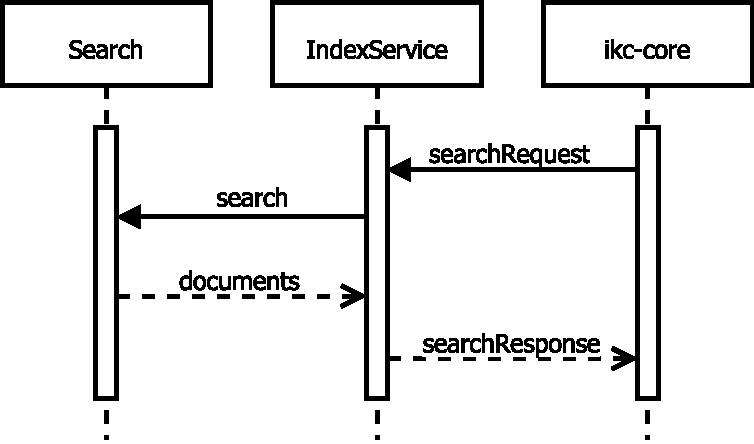
\includegraphics[width=0.7\textwidth]{SeqSearch}
    \caption{Ablauf: Suche}
    \label{fig:seqsearch}
    \end{figure}

\begin{listing}[H]
\inputminted[
frame=lines,
framesep=2mm,
baselinestretch=1.2,
linenos,
breaklines=true
]{js}{sourcecode/IndexService/search.ts}
\caption{Suche}
\label{search}
\end{listing}

% ----------------------------------------------------------------

\section{DataService}

% ----------------------------------------------------------------

Der \texttt{DataService} versorgt den \gls{ikc-core} und den \texttt{IndexService} mit den essentiellen Daten. Diese beinhalten die Textquellen an sich aber auch die verschiedenen Indizes. Diese werden über \gls{SSH} per \gls{SFTP} von einer externen Datenquelle angefordert und anschliessend bereitgestellt. 

    \begin{figure}[H]
    \centering
    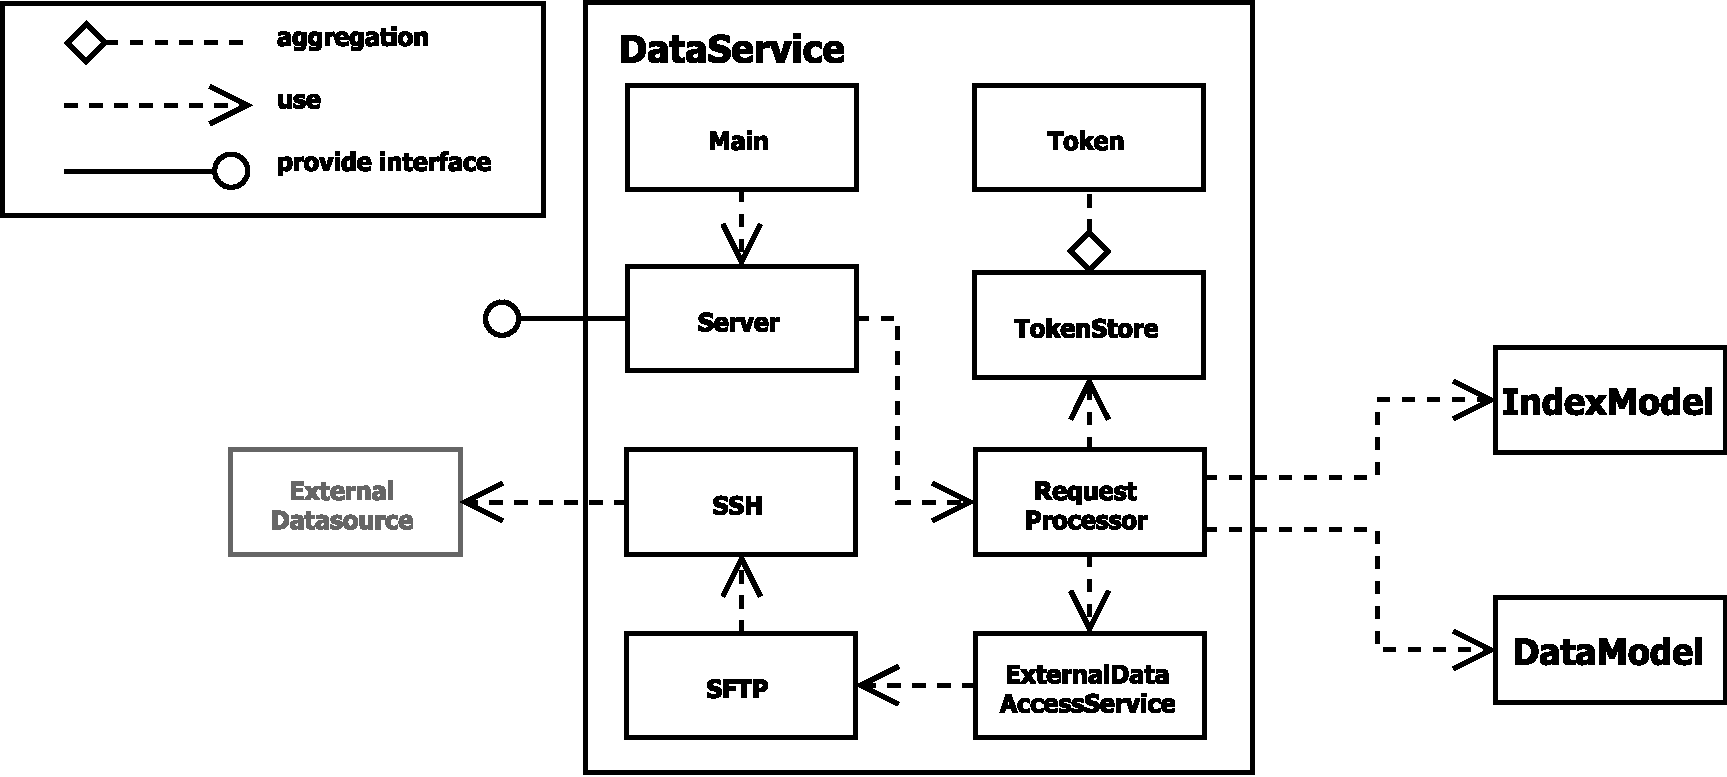
\includegraphics[width=1\textwidth]{DataServiceClassDiagram}
    \caption{DataService Klassendiagram}
    \label{fig:dataserviceClassDiagram}
    \end{figure}


\begin{itemize}
    \item \textbf{Main}: Die ist die Startklasse des DataService. Sie initialisiert und startet den Server und alle weiteren nötigen Services.
    \item \textbf{Server}: Auch hier hat der \texttt{Server} wiederum die Aufgabe Anfragen entgegenzunehmen und zu beantworten.
    \item \textbf{RequestProcessor}: Der \texttt{RequestProcessor} ist die Hauptklasse. Hier ist die zentrale Applikationslogik enthalten, Anfragen werden weitergeleitet. Die Anbindungen an eine Datenquelle werden ebenfalls von hier aus gesteuert.
    \item \textbf{ExternalDataAccessService}: Diese Klasse kapselt den Zugriff auf externe Datenquellen. Im Diagramm stellt sie die Verbindung zu einem \gls{SFTP}-Server bereit.
    \item \textbf{TokenStore}: Das Zugriffskonzept mittels \gls{Token}[s] benötigt eine Zwischenspeicherung der Freigabeberechtigungen. Dies findet hier statt. 
    \item \textbf{Token}: Diese Klasse repräsentiert eine Zugriffberechtigung innerhalb des DataService.
    \item \textbf{SFTPService}: Ein Beispiel für eine externe Datenquelle ist \gls{SFTP}. Da der Zugriff hierbei über \gls{SSH} zu erfolgen hat, fungiert diese Klasse hier als Adapter.
    \item \textbf{SSHService}: Hier findet der eigentliche Zugriff auf die externe Datenquelle statt. Die Kommunikation geschieht über einen \gls{SSH}-Tunnel.
\end{itemize}

\subsection{Grundaufbau}

Die Grundlage des DataServices bildet der Server. Dieser ist verantwortlich für die Netzwerkverbindungen zum IndexService und dem \gls{ikc-core}. Der \autoref{server.ts} zeigt die Initialisierung des Sockets und die Delegation von Anfragen. Auf Zeile 26 wird ein stan\-dard\-mäs\-siger HTTP-Server instanziiert. Dieser wird auf Zeile 27 als Basis für von Socket.io zur Verfügung gestellten Server benutzt. Der Server nimmt Anfrage auf einem bestimmten Port (Zeile 28) entgegen. Die Methode \verb|waitForConnection| (Zeile 32) nimmmt eingehende Anfragen entgegen. Haben diese Anfragen eine bestimmte Route als Ziel (Zeile 34), werden diese zur Methode \verb|processRequest| weitergeleitet. \verb|ss| ist eine Instanz von socket.io-stream. Die Anfragen werden somit direkt als \gls{Stream} entgegengenommen.

\begin{listing}[H]
\inputminted[
frame=lines,
framesep=2mm,
baselinestretch=1.2,
linenos,
breaklines=true,
firstline=25,
lastline=38
]{js}{sourcecode/dataservice/Server.ts}
\caption{Grundaufbau}
\label{server.ts}
\end{listing}

Nun beginnt die eigentliche Verarbeitung der Anfrage (siehe \autoref{server2.ts}). Der \autoref{server2.ts} zeigt die weiteren Schritte: \verb|processRequest| (Zeile 40) nimmt den \gls{Stream} und die \gls{Websocket} entgegen. Weiter konvertiert die Funktion \texttt{stream\-To\-Da\-ta} des Moduls \verb|StreamingHelper| den \gls{Stream} zur weiteren Verarbeitung zu Daten. Ist diese Arbeit getan, wird das \gls{Callback} aufgerufen, worin der \gls{Stream}, die Daten und der \gls{Websocket} an die Methode \verb|processPayload| weitergegeben werden. Hier (Zeile 47) wird der \texttt{MessageMangager} (siehe \autoref{s-message-manager}) genutzt, um die eingetroffene Nachricht entsprechend weiter zu verarbeiten. Kurz erklärt, der \texttt{MessageManager} entkoppelt die Kommunikation von der eigentlichen Verarbeitung der jeweiligen Nachricht. Das Resultat wird mittels \texttt{prepareMessage} auf Zeile 52 weiter verarbeitet. Der \texttt{Stream\-ing\-Help\-er} kümmert sich wiederum um das Verpacken der Daten in einen \gls{Stream}. Schlussendlich wird die Nachricht auf Zeile 59 verschickt. Dies geschieht über den socket.io-stream mittels der Methode \texttt{emit} und wiederum über den Bezeichner \verb|'route'|.


\begin{listing}[H]
\inputminted[
frame=lines,
framesep=2mm,
baselinestretch=1.2,
linenos,
breaklines=true,
firstline=40, lastline=62]{js}{sourcecode/dataservice/Server.ts}
\caption{Verarbeitung}
\label{server2.ts}
\end{listing}


% ----------------------------------------------------------------

\subsection{AccessSession}

% ----------------------------------------------------------------

Die \texttt{AccessSession} ist die Zugangsberechtigung in Codeform. Das Interface im \autoref{access-session-interface.ts} zeigt die mindestens notwendigen Eigenschaften, sodass ein Zugang möglich ist. Dafür nötig sind ein Typ der \texttt{AccessSession} zur Identifikation und eine Sammlung von Pfadbeschreibungen.

\begin{listing}[H]
\inputminted[
frame=lines,
framesep=2mm,
baselinestretch=1.2,
linenos,
breaklines=true,
firstline=19,
lastline=22
]{js}{sourcecode/dataservice/AccessSession.ts}
\caption{Interface: AccessSession}
\label{access-session-interface.ts}
\end{listing}

Der \autoref{path-desc} zeigt die Klasse einer solchen Pfadbeschreibung. Diese wiederum enthält alle Informationen zur Auffindung von einer einzelnen oder mehreren Dateien. Die Eigenschaft \texttt{path} hält den Pfad zum Ort, wo gesucht werden soll. Dies ist zum Beispiel ein Ordner auf einem entfernten Server. \texttt{searchPattern} dient der Suche nach der Datei oder vor allem der Dateien. Mittels Platzhaltern in Form von \texttt{*} können beliebige Dateien, welche aber beispielsweise einem Muster entsprechen zurückgegeben werden. \verb|**/*.txt| würde alle Textdateien in einem Unterordner betreffen. Die letzte Eigenschaft \texttt{referenceFilePath} enthält den Pfad zu einer Datei. Diese dient mit ihrem Änderungsdatum als Referenz für die restlichen Dateien oder die restliche Datei. Der \autoref{auto-indexierung} zeigt eine mögliche Anwendung mithilfe dieser Referenz.

\begin{listing}[H]
\inputminted[
frame=lines,
framesep=2mm,
baselinestretch=1.2,
linenos,
breaklines=true,
firstline=43,
lastline=48
]{js}{sourcecode/dataservice/AccessSession.ts}
\caption{PathDescription}
\label{path-desc}
\end{listing}



% ----------------------------------------------------------------

\section{Kommunikation}

% ----------------------------------------------------------------

Die Kommunikation zwischen den verschiedenen Services und Komponenten ist ein kritischer Faktor für die generelle Performance des gesamten Systems. Einerseits werden sehr viele Dateien über das Netz\-we\-rk übermittelt, andererseits muss auch damit ge\-rech\-net werden, dass einzelne Dateien Dateigrössen von bis zu 200 Megabyte überschreiten.

% ----------------------------------------------------------------

\subsection{Identifizierte Probleme}

% ----------------------------------------------------------------

Während der ersten Testimplementationen waren kritische Punkte schnell gefunden. Die Übermittelung von sehr vielen und auch grossen Dateien benötigt zusätzlichen Aufwand.

\begin{enumerate}
    \item \textbf{Umgang mit grossen Dateien:} Die grossen Dateien können auf\-grund Begrenzungen des Arbeitsspeichers und oder Be\-grenz\-ung der Datentypen nicht ohne weitere Schritte verwendet werden. Eine Lösung dafür ist die Verwendung von \gls{Stream}[s] und \gls{Buffer}[s].
    \item \textbf{Parsen und Serialisieren:} Die Übersetzung von rohen Bi\-när\-da\-ten in ein Objekt und umgekehrt, ist bei grossen Dateien ebenfalls nicht trivial. \texttt{JSON.parse} und {JSON:stringify} funktionieren nicht ohne Weiteres.
\end{enumerate}

Für die Verwendung wurden diverse Zusatzbiblbioteheken geprüft. Für die finale Implementation wurden folgende eingesetzt:

\texttt{socket.io}\footnote{\url{https://github.com/socketio/socket.io/}} ist eine viel versprechende Bibliothek. Sie ist in praktisch allen gängigen Programmiersprachen implementiert, darum gibt es auch zahlreiche Erweiterungen. Ebenfalls gibt es eine Erweiterung für die Verwendung von \gls{Stream}[s] namens \texttt{socket.io-stream}\footnote{\url{https://github.com/nkzawa/socket.io-stream}}.

Für die Serialisierung und das Parsen wird zusätzlich \texttt{msgpack}\footnote{\url{http://msgpack.org}} verwendet. Es arbeitet problemlos mit grossen Dateien und ist gleichzeitig sehr performant.

Die \autoref{fig:kommunikation} zeigt die schlussendlich verwendeten Technologien im Überblick. Die Grundlage der Kommunikation zwischen \gls{ikc-core}, \texttt{DataService} und \texttt{IndexService} bildet \texttt{TCP/IP}. Darüber läuft das abhörsichere \texttt{HTTPS}-Protokoll. Im \texttt{JavaScript} wird die Bibliothek \texttt{socket.io} mit der oben erwähnten \gls{Stream}-Erweiterung verwendet. \texttt{msgpack} übersetzt die binären Rohdaten in Objekte und umgekehrt.

    \begin{figure}[H]
    \centering
    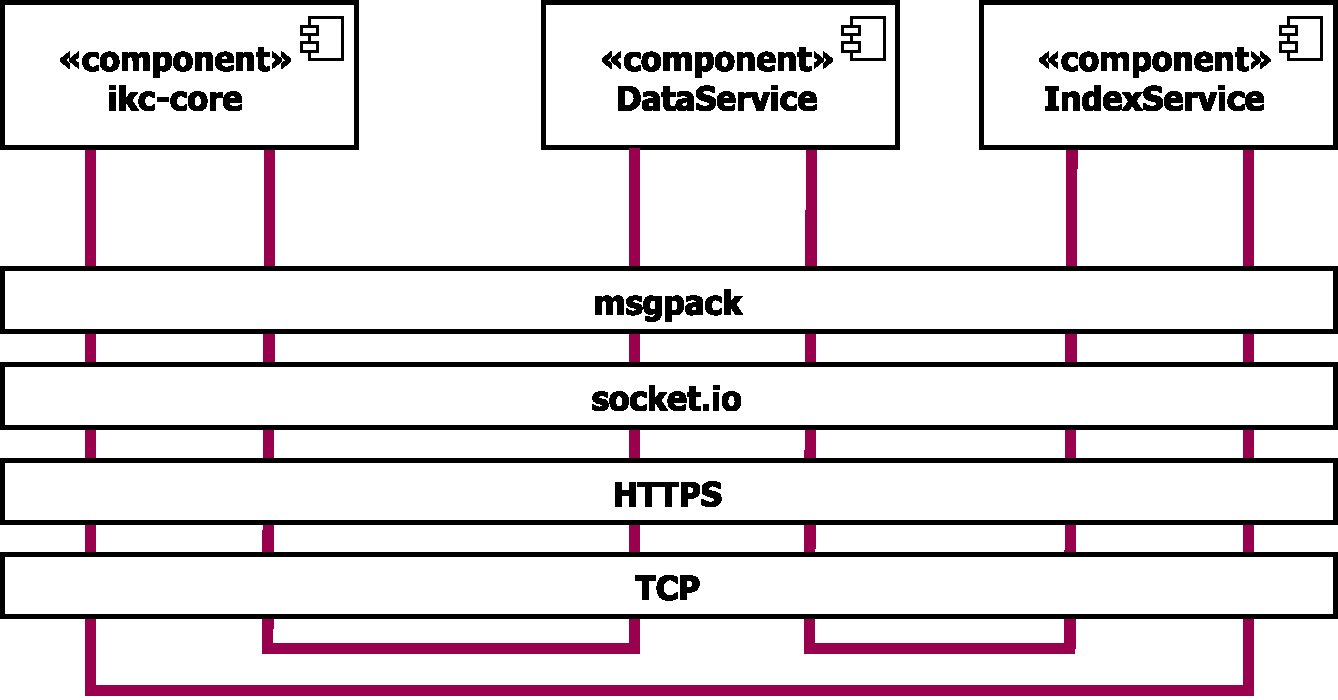
\includegraphics[width=1\textwidth]{ComponentDiagramm}
    \caption{Kommunikation}
    \label{fig:kommunikation}
    \end{figure}
    
% ----------------------------------------------------------------

\subsection{Protokoll}\label{section:protokoll}

% ----------------------------------------------------------------

Das Protokoll gibt an, in welchem Format die Daten übermittelt werden, sodass sie von beiden Seiten korrekt interpretiert werden. Es setzt also noch eine zusätzliche Ebene auf das obige Diagramm (\autoref{fig:kommunikation}).


%    \begin{figure}[ht]
%    \centering
%    
\includegraphics[width=0.5\textwidth]{Protocol}
%    \caption{Protokoll Aufbau}
%    \label{fig:protocol}
%    \end{figure}

Die Kommunikation mit dem \texttt{IndexService} und dem \texttt{DataService} verläuft komplett eigenständig. Darum verwenden beide Services ein eigenes Protokoll. Für die Kommunikation mit einem Service muss das jeweilige Protkoll auch von der Gegenseite eingesetzt werden. Die Bedingung ist, dass alle zu übermittelnden Daten eine Instanz einer Klasse aus dem jeweiligen Protokoll sind.
    
%Diagramm Ablauf ala \url{http://www.hsg-kl.de/faecher/inf/netze/fehler2/index.php} 
%Diagramm Stack oder level evt. mit Diagramm kabel mit verschiedenen schichten oder standard protocol stack \url{https://www.google.ch/url?sa=i&rct=j&q=&esrc=s&source=images&cd=&ved=0ahUKEwjJ5uO57drTAhUGvRoKHZIbBE4QjhwIBQ&url=http%3A%2F%2Fgeti2p.net%2Fnl%2Fdocs%2Fprotocol&psig=AFQjCNEHKXFjqJgGFF7pzQhblQm2WwWp6w&ust=1494145920025872}

Grundsätzlich besteht jede Nachricht aus einem Objekt der abstrakten Klasse \texttt{Mes\-sa\-ge}. Es stammt vorzugsweise aus der \texttt{MessageFactory}, um die Erzeugung des Objektes zusätzlich zu entkoppeln. Eine \texttt{Mes\-sa\-ge} besteht immer aus 

\begin{itemize}
    \item \textbf{\texttt{UUID}}:
    Diese identifiziert eine Nachricht eindeutig. Sie besteht aus einem zufällig generierten alphanumerischen Muster.
    \item \textbf{\texttt{MessageType}}:
    Damit die Nachricht jederzeit und an allen dafür vorgesehen Orten richtig interpretiert werden kann, besitzt sie einen für den jeweiligen Zweck vorgesehenen Typ. Dieser gibt explizit an, wie die Nachricht aufgebaut ist und welchen Zweck sie hat.
    \item \textbf{\texttt{Messagebody}}:
    Dieser stellt der eigentliche Inhalt der Nachricht dar. Er enthält den für den jeweiligen Typ vorgesehenen Body.
\end{itemize}

Das Klassendiagramm (\autoref{fig:messageClassDiagram}) zeigt den Aufbau der abstrakten Klasse \texttt{Message} noch etwas detaillierter auf. Wie man erkennen kann, handelt es sich beim \texttt{MessageBody} um ein \texttt{Interface}, beim \texttt{MessageType} um einen \texttt{Enumerator}. Der \texttt{MessageBody} kann somit jeweils eine für den Zweck passende Instanz halten. Eine abstrakte Klasse wird aus dem Grund eingesetzt, dass die \texttt{id} zwingend bei jeder Unterklasse gesetzt wird.

    \begin{figure}[H]
    \centering
    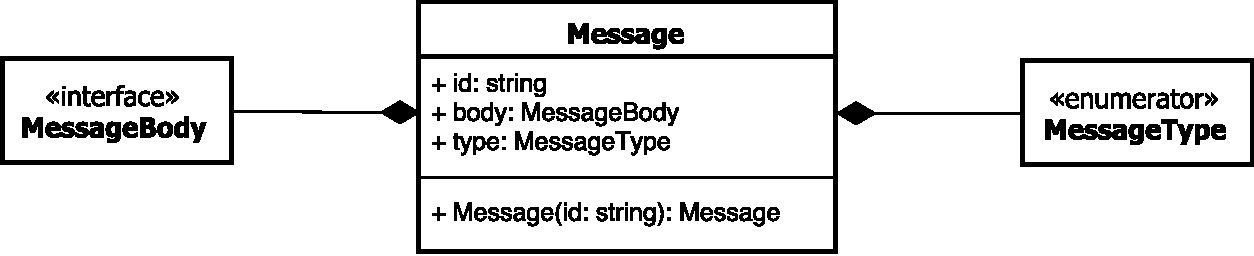
\includegraphics[width=1\textwidth]{MessageClassDiagram}
    \caption{Message Klassendiagramm}
    \label{fig:messageClassDiagram}
    \end{figure}


% ----------------------------------------------------------------

\subsection{DataService-Protokoll}

% ----------------------------------------------------------------

\autoref{fig:dataclass} zeigt den Aufbau des \texttt{DataService}-Protokolls, dieses liegt im eigenen Paket \texttt{DataModel}. Dieses Protokoll wird im Prototyp für die Kommunikation zwischen \gls{ikc-core} und \texttt{DataService} beziehungsweise \texttt{IndexService} und \texttt{DataService} verwendet.

Im obigen Abschnitt (\autoref{section:protokoll}) wurde der Grundaufbau einer Nachricht aufgezeigt. Das \texttt{DataService}-Protokoll wird prinzipiell für den Datentransport eingesetzt. Das Protokoll gibt die dafür zu verwendenden Typen (\texttt{MessageType}) und Bodies (\texttt{MessageBody}) an. Die folgende Tabelle gibt einen Überblick über die verschiedenen Optionen. Zusätzlich zeigt das Ablaufdiagramm (\autoref{fig:seqdataprotocol}) einen vorstellbaren Beispielablauf mit den beteiligten Komponenten \gls{ikc-core} und \texttt{DataService}. Grundsätzlich folgt auf einen \texttt{Request} stets die entsprechende \texttt{Response}. Davon ausgenommen ist der Fehlerfall, wobei eine \texttt{ErrorResponse} zurückgeliefert wird.

\begin{longtable}{|p{4cm}| p{8cm}|}
  \hline
    \textbf{Bezeichnung} & \textbf{Beschreibung}\\\hline
    \texttt{TokenRequest} & Hierbei geht es um die Anfrage für eine Freigabe einer Datei oder eines Verzeichnisses. Für diesen Zweck gibt es das \texttt{Interface} \texttt{AccessSession}. Es enthält alle nötigen Zugangsdaten zur Verbindung mit einer externen Datenquelle. \newline
    
    Im Diagramm (\autoref{fig:seqdataprotocol}) ist die Klasse \texttt{SFTPAccessSession} enthalten. Diese regelt als Beispiel den Zugriff auf einen SFTP-Server.
    \\\hline
    \texttt{TokenResponse} &    
    Hat der \texttt{DataService} die Anfrage erhalten, schickt dieser bei Erfolg einen Token zurück. Dies geschieht in Form der \texttt{TokenResponse}. Diese enthält einen \gls{Token}. Er ist eine einmalige Zugriffsfreigabe für eine Datei oder einen Ordner von der jeweiligen Datenquelle.\newline
    
    
    Der \gls{Token} ist ein zufälliger generierter String, welcher auf dem \texttt{DataService} mit der jeweiligen \texttt{AccessSession} abgelegt ist.\\\hline
    \texttt{DataRequest} & Auf eine \texttt{TokenResponse} folgt ein \texttt{DataRequest}. Ist ein \gls{Token} auf dem \texttt{DataService} hinterlegt, kann mit Hilfe dieses innerhalb eines \texttt{DataRequests} die jeweilige Datei oder das jeweilige Verzeichnis angefragt werden. \\\hline
    \texttt{DataResponse} & Die Antwort auf einen \texttt{DataRequest} ist im besten Fall eine \texttt{DataResponse}. Diese enthält den angefragten Dateiinhalt. \\\hline
    \texttt{ErrorResponse} & Schlägt bei einer der obigen Anfragen etwas fehl, wird eine \texttt{ErrorResponse} mit dem jeweiligen Fehler zurückgegeben. Fehlerursachen können von sehr unterschiedlicher Natur sein, beispielsweise sind Netzwerkprobleme oder falsche Zugangsdaten vorstellbar.\\\hline
        \caption{DataService: Message-Klassen}
    \label{dataservice-bodies}
\end{longtable}


    \begin{figure}[H]
    \centering
    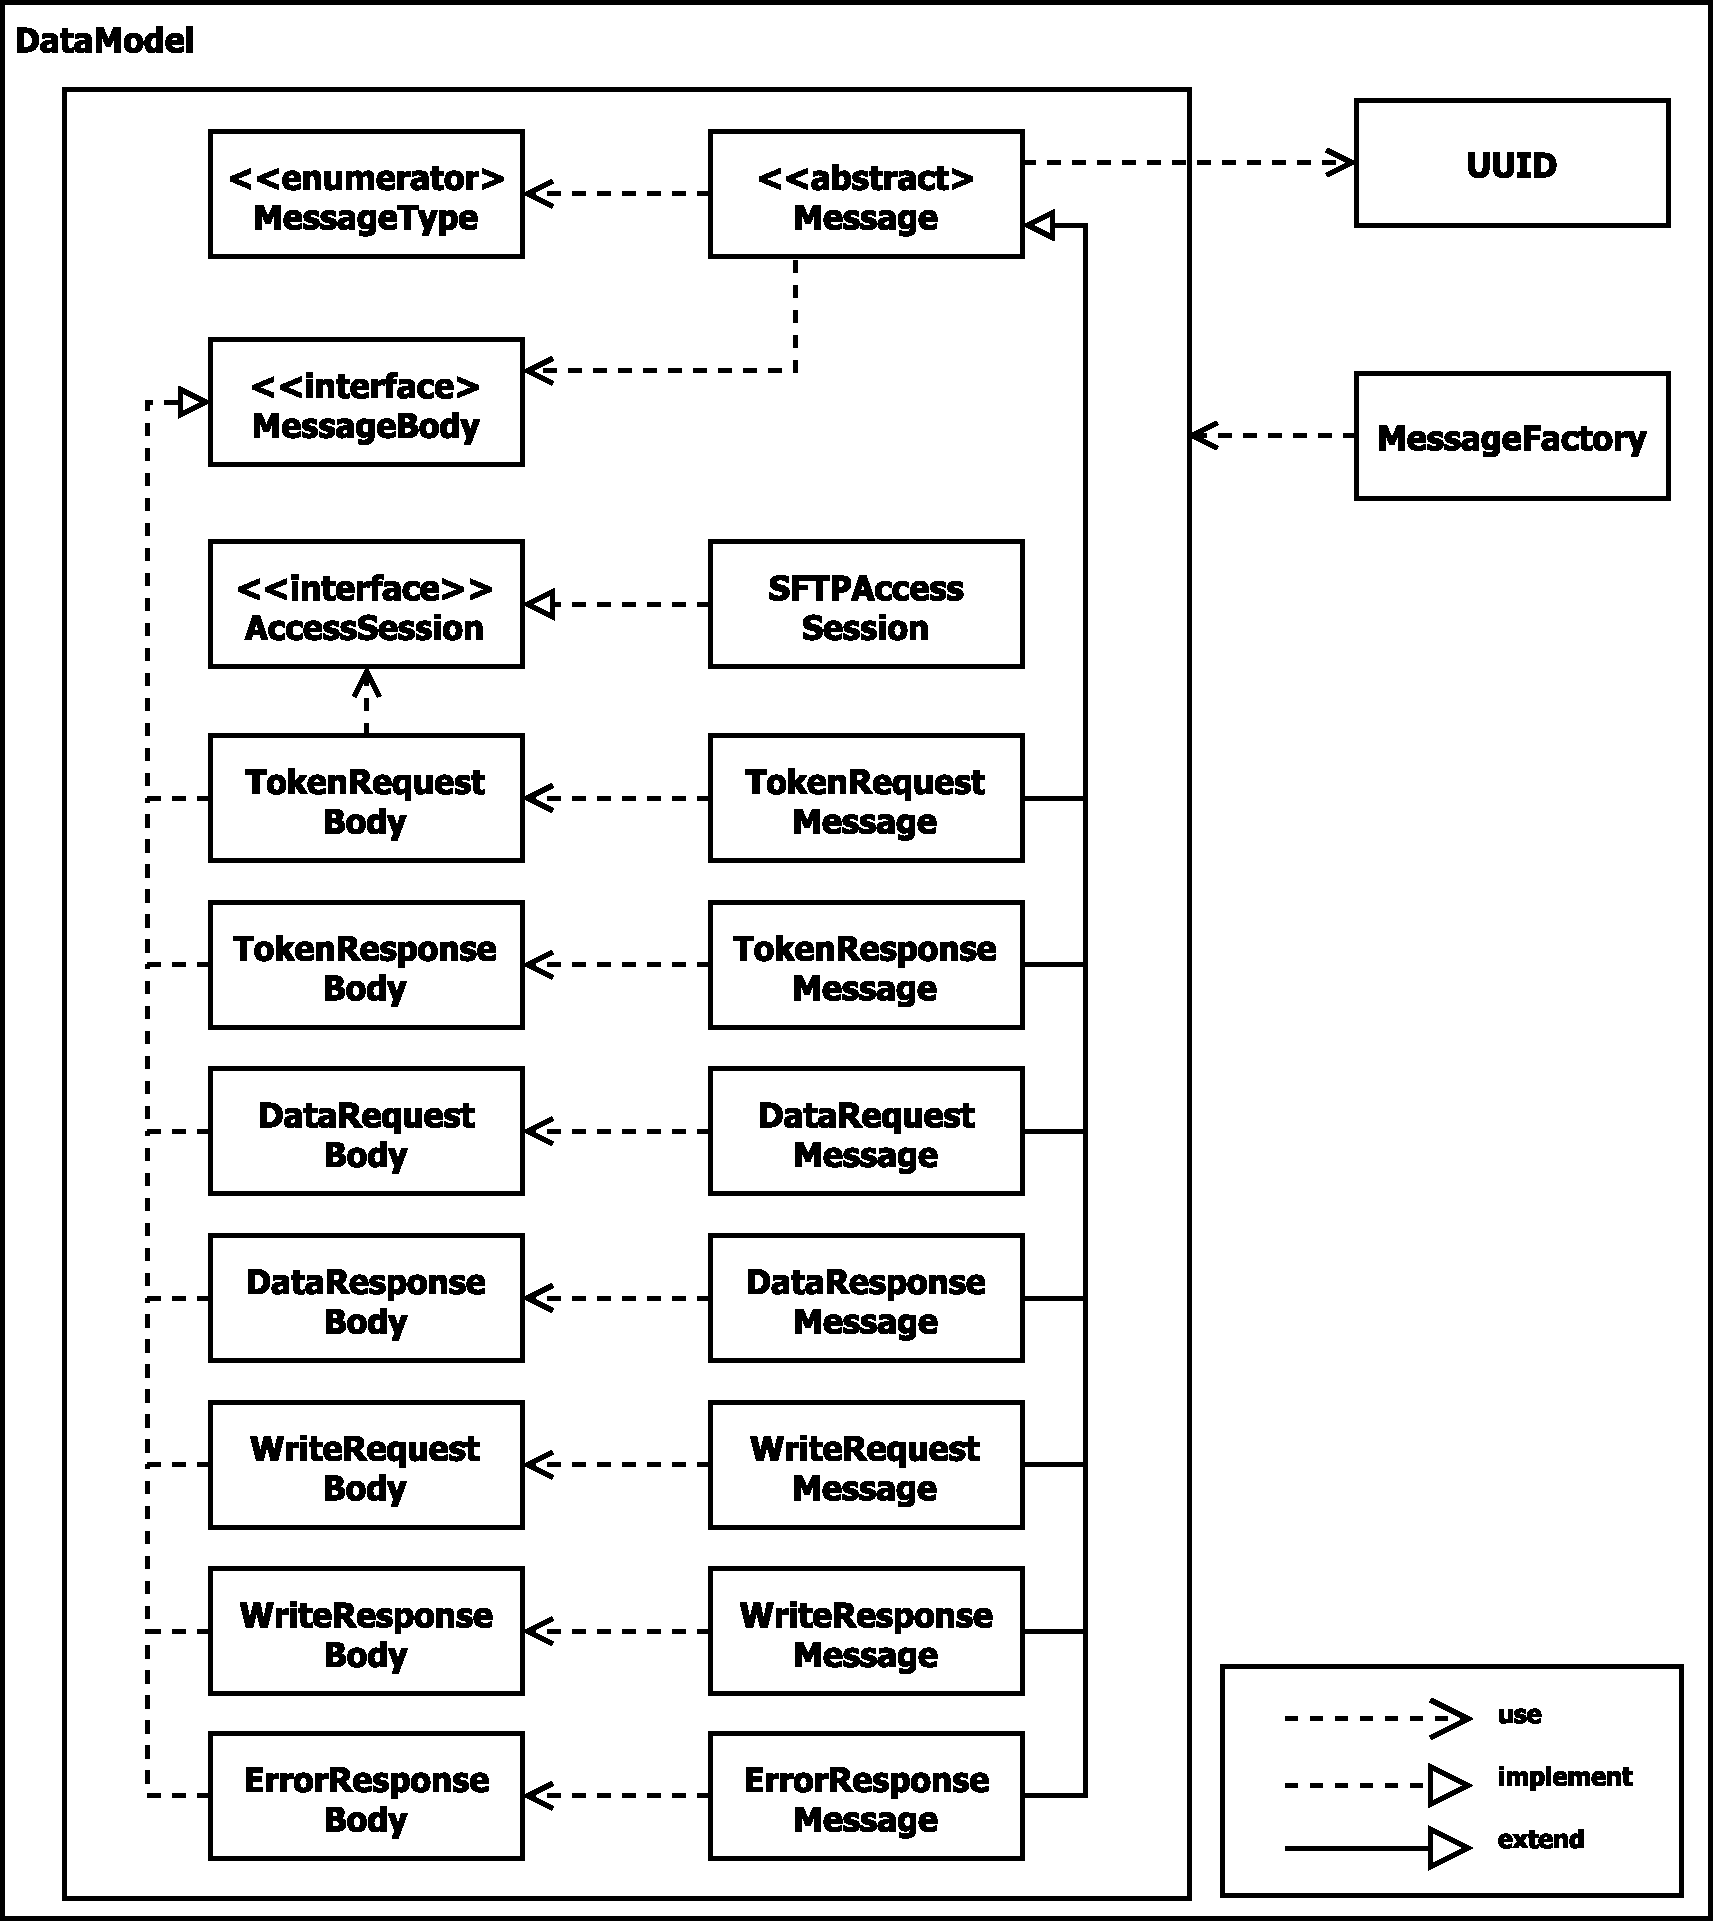
\includegraphics[width=0.9\textwidth]{DataModelClassDiagramm}
    \caption{Klassendiagramm DataService-Protokoll}
    \label{fig:dataclass}
    \end{figure}

    \begin{figure}[H]
    \centering
    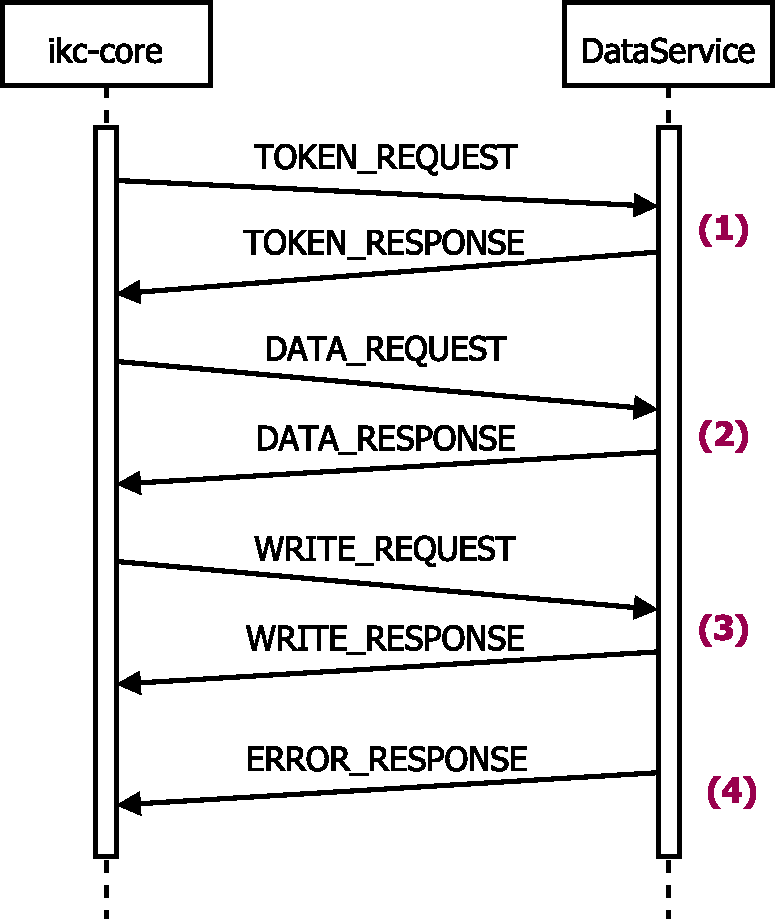
\includegraphics[width=0.5\textwidth]{DataModelSequence}
    \caption{Ablauf DataService-Protokoll}
    \label{fig:seqdataprotocol}
    \end{figure}

% ----------------------------------------------------------------

\subsection{IndexService-Protokoll}

% ----------------------------------------------------------------

Vom Aufbau her ähnlich wie das \texttt{DataService}-Protokoll sieht auch das \texttt{IndexService}-Protokoll aus (\autoref{fig:indexclass}). Wiederum ist die abstrakte Klasse \texttt{Message} die Grundlage. Allerdings unterscheiden sich die \texttt{Mes\-sa\-ge\-Typ\-es} und \texttt{MessageBodies}. Die Nachrichten haben hier den Zweck, alle für die Volltextsuche und die Schlüs\-sel\-wort-\-Ex\-trak\-tion erforderlichen Daten zur Verfügung zu stellen.

    
    \begin{figure}[H]
    \centering
    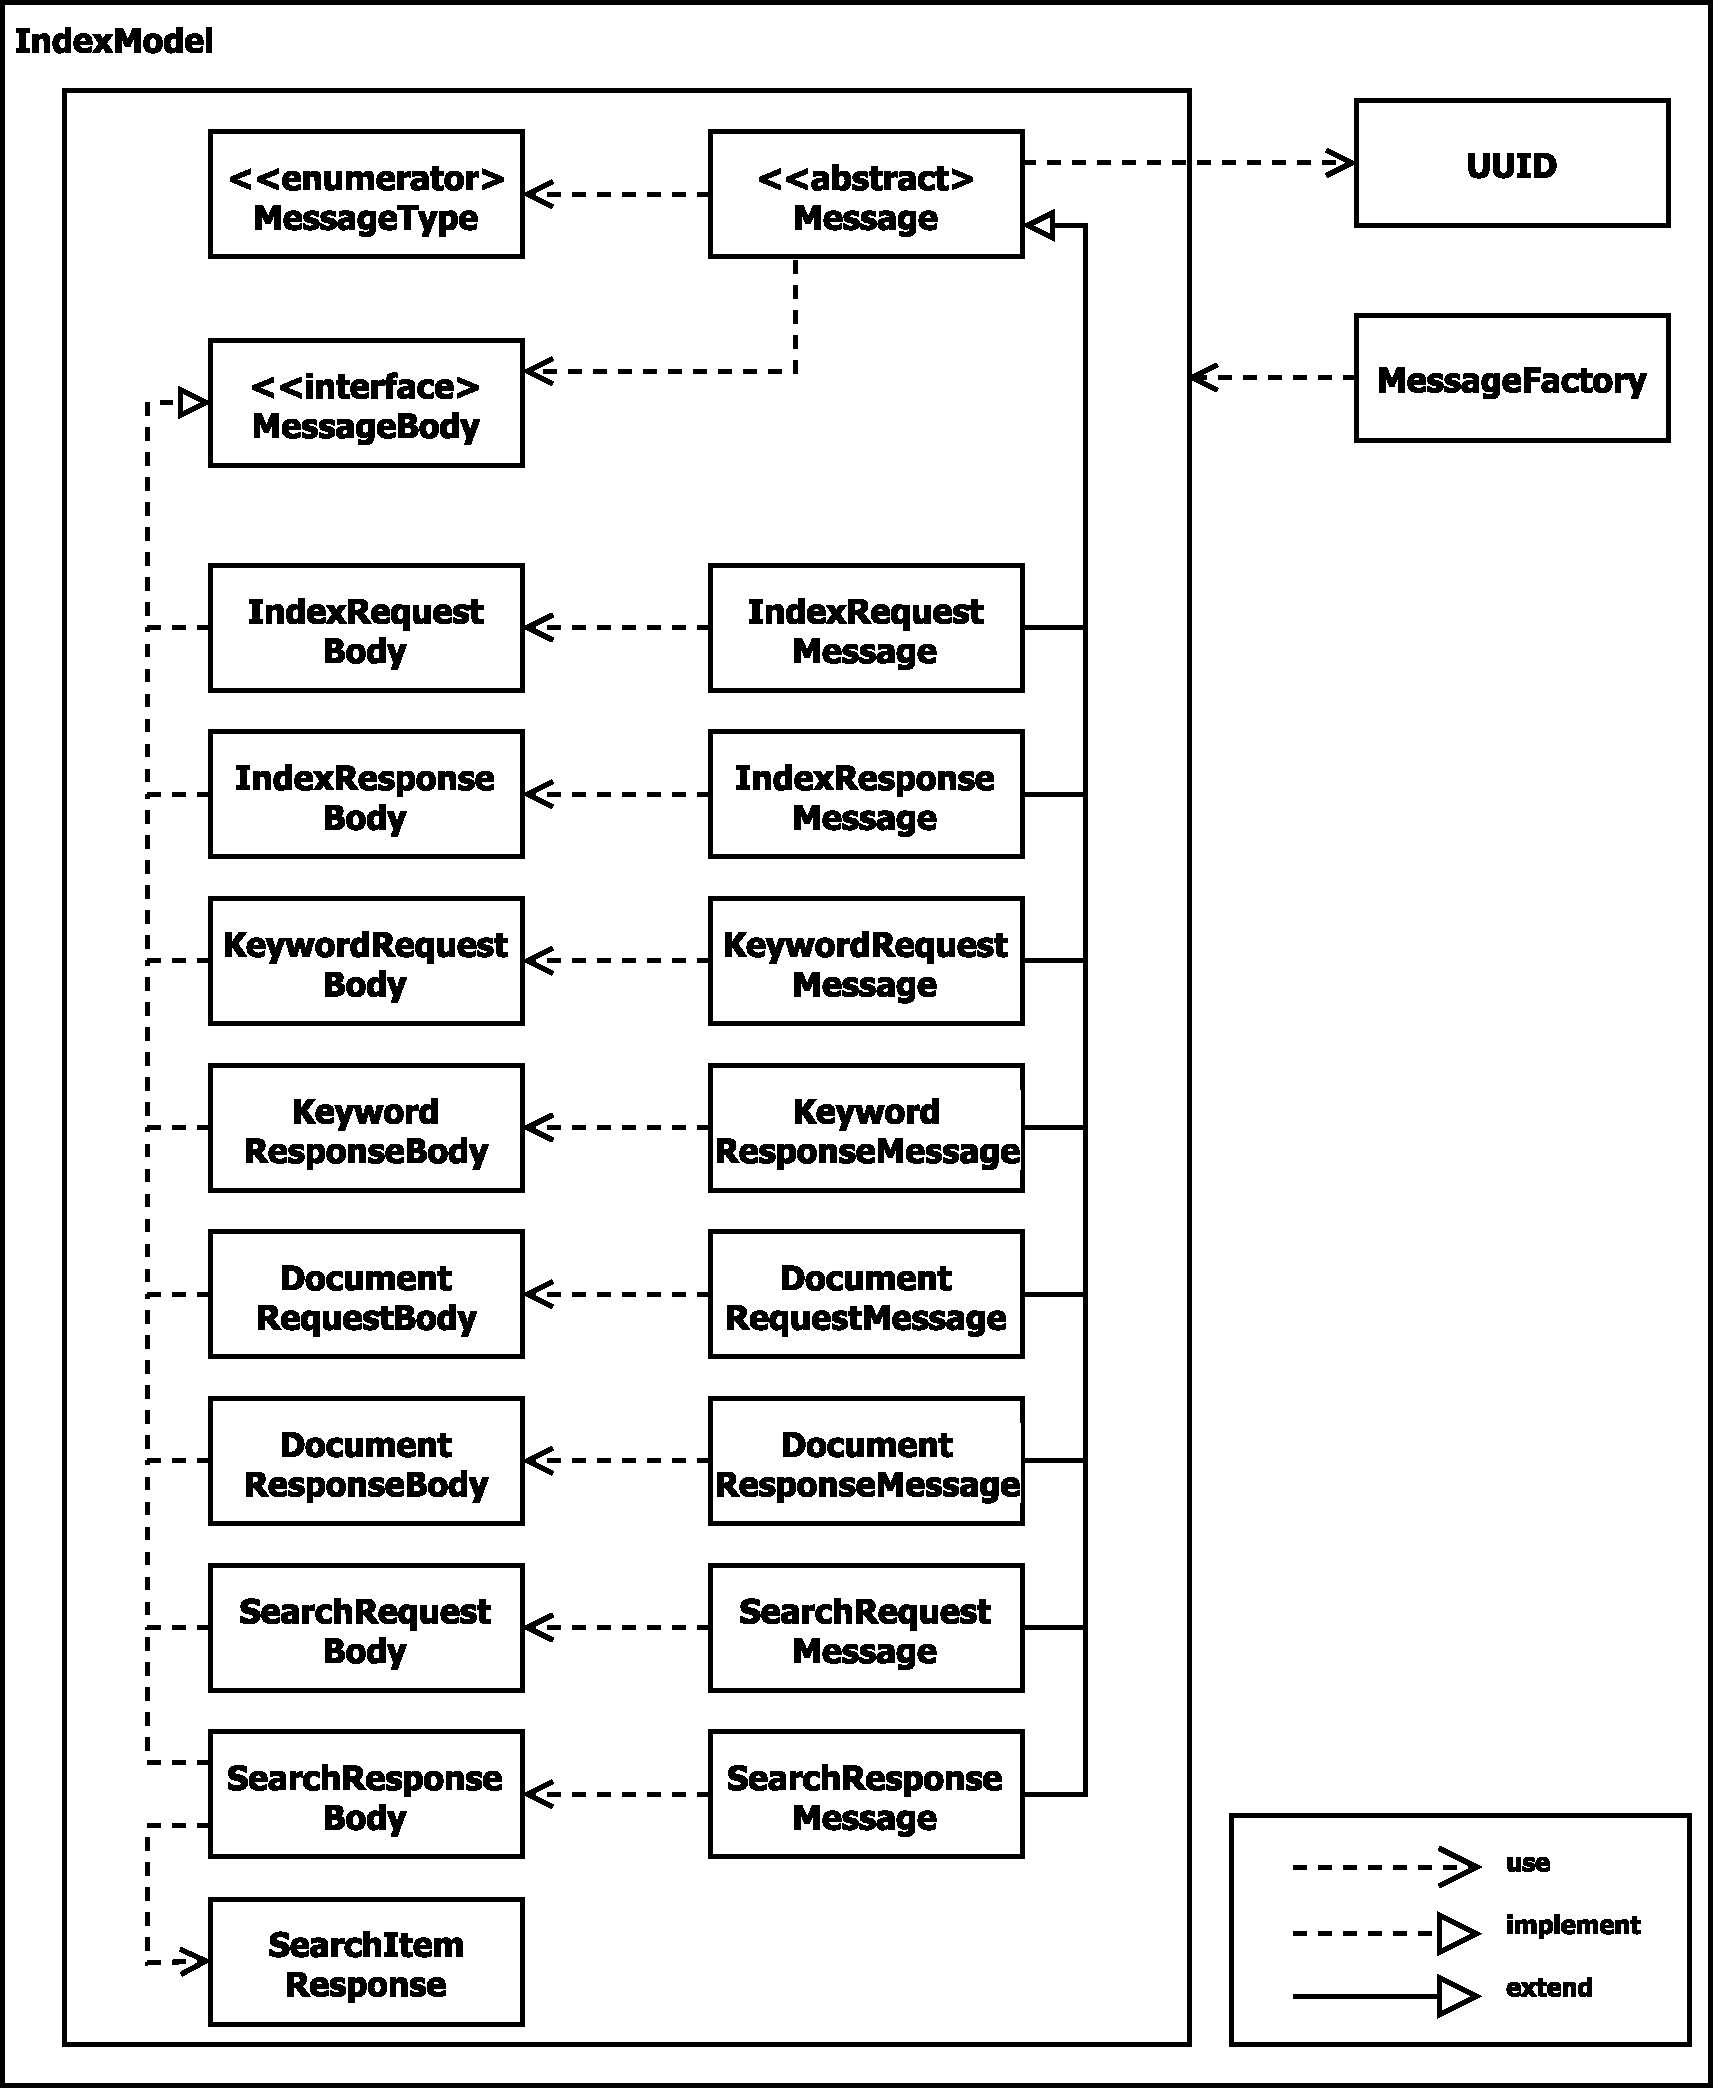
\includegraphics[width=1\textwidth]{IndexModelClassDiagramm}
    \caption{Klassendiagramm IndexService-Protokoll}
    \label{fig:indexclass}
    \end{figure}

Die Grundlage für die weiteren Vorgänge ist der Volltextindex. Dieser kann gelesen und persistiert werden. Ist diese Voraussetzung gegeben, können Schlüsselwörter für ein Dokument angefragt, zu einem Schlüsselwort passende Dokumente gefunden und Suchresultate für einen bestimmten Begriff ermittelt werden. Die Abläufe sind in der \autoref{fig:seqindexprotocol} ersichtlich. Die Vorgänge werden in folgender Tabelle genauer erläutert.

\begin{longtable}{|p{4cm}| p{8cm}|}
  \hline
    \textbf{Bezeichnung} & \textbf{Beschreibung}\\\hline
    \texttt{IndexRequest} & Der \texttt{IndexRequest} dient zum Anfragen des Volltextindex. Für diesen Vorgang wird zunächst der \gls{Token}, welcher zuvor beim \texttt{DataService} angefragt wurde, mitgeliefert. Zusätzlich dazu liegt der \texttt{Host} des anzufragenden \texttt{DataService}. Die \texttt{indexId} ist die Identifikationsnummer des Index, falls dieser schon zuvor angefragt wurde.\\\hline
    \texttt{IndexResponse} & Nach der vorgängigen Anfrage für einen Index, folgt die Antwort in Form einer \texttt{IndexResponse}. Einziger Inhalt ist die \texttt{indexId} in Form eines Strings, welche den Index eindeutig identifizierbar macht.\\\hline
    \texttt{KeywordRequest} & Für die Schlüsselwort-Extraktion werden die Schlüsselwörter eines jeden Dokuments benötigt. Dafür gibt es den Vorgang \texttt{KeywordRequest}. Für die Verarbeitung werden ein \texttt{token} und ein \texttt{indexId} mitgeliefert. Der \texttt{token} hat seinen Ursprung wiederum im \texttt{DataService}. Er dient dazu den Volltext der jeweiligen Datei anzufragen. Die \texttt{indexId} ist wiederum dazu da, den gewünschten Index zu identifizieren.\\\hline
    \texttt{KeywordResponse} & Nach der obigen Anfrage folgt die Antwort in Form einer \texttt{KeywordResponse}. Diese beinhaltet ein Array von Strings, welches die extrahierten Schlüsselwörter des Dokumentes beinhaltet und die Identifikationsnummer des jeweiligen Dokumentes.\\\hline
    \texttt{DocumentRequest} & Sollen zu einem Schlüsselwort passende Dokumente angefragt werden, wird der \texttt{DocumentRequest} benutzt. Diese Anfrage beinhaltet das gesuchte Schlüsselwort und die Identifikationsnummer des jeweiligen Index.\\\hline
    \texttt{DocumentResponse} & Die Antwort beinhaltet wiederum das zuvor gesuchte Schlüsselwort und die Resultate als Array von Resultaten. Ein Resultat enthält den Titel, den Pfad, die Identifikationsnummer und den Inhalt des Dokumentes im Volltext.\\\hline
    \texttt{SearchRequest} & Eine weitere Funktionalität ist die Volltextsuche. Auch für diesen Zweck gibt es wiederum eine eigene Klasse. Um eine Suchanfrage abzusetzen, wird der Suchbegriff, eine Suchanfrage-Identifikationsnummer und wiederum eine \texttt{indexId} benötigt.\\\hline
    \texttt{SearchResponse} & Als Antwort auf eine Suchanfrage folgt ein Array von Suchresultaten. Ein Suchresultat enthält die Identifikationsnummer, den Pfad, den Titel und den Inhalt des gefundenen Dokuments.\\\hline
        \caption{IndexService: Message-Klassen}
    \label{indexservice-bodies}
\end{longtable}

    \begin{figure}[H]
    \centering
    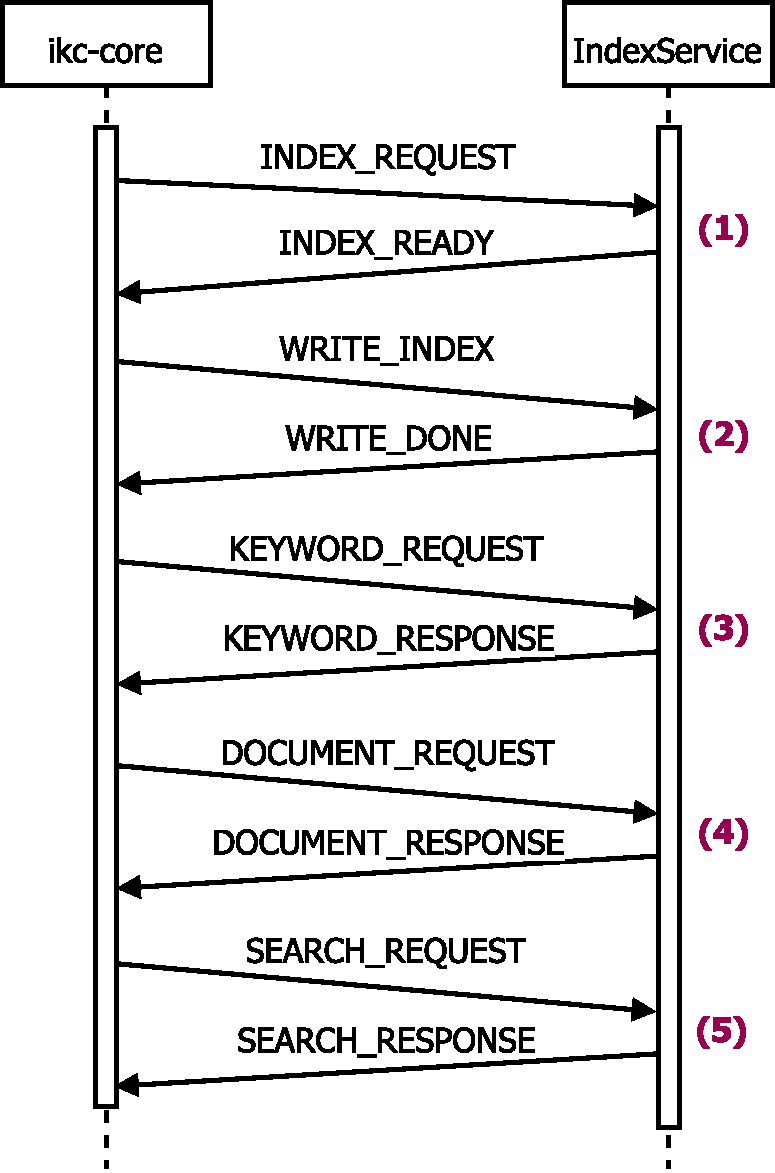
\includegraphics[width=0.5\textwidth]{IndexModelSequence}
    \caption{Ablauf IndexService-Protokoll}
    \label{fig:seqindexprotocol}
    \end{figure}

% ----------------------------------------------------------------

\section{Daten}

% ----------------------------------------------------------------

Die Daten sind die Grundlagen dieser Arbeit und spielen deshalb eine wichtige Rolle im gesamtem Projektverlauf. Insbesondere die Persistenz und auch die Freigabe von Daten sind grundlegende Bestandteile der Implementation.


% ----------------------------------------------------------------
    
\subsection{Quelle}

% ----------------------------------------------------------------


Als Datenquelle wird eine vom Auftraggeber zur Verfügung gestellte Sammlung von etwas mehr als 100'000 Wikipedia Artikeln verwendet. Diese enthalten qualitativ hochwertige Informationen in Volltext und bilden die Grundlage für die Schlüsselwort-Extraktion und die Volltextsuche.

% ----------------------------------------------------------------

\subsection{Persistenz}

% ----------------------------------------------------------------


Im Gegensatz zum bestehenden Prototypen aus dem Forschungsprojekt \gls{IKC}, wird in dem hier vorliegenden als Datenquelle zusätzlich \gls{SFTP} ergänzt. Dies hat mitunter den Grund, wie in Absprache mit dem Auftraggeber festgelegt wurde, dass die erweiterte Anbindung an Cloud-Dienste, wie etwa Dropbox und Evernote, nicht der Kern dieser Bachelor-Arbeit ist. Der Fokus dieser Arbeit ist \textit{Information Retrieval} mittels \textit{Natural Language Processing} auf Basis von Schlüsselwort-Extraktion. Daher soll auch in diesem Bereich der Grossteil der zur Verfügung stehenden Zeit investiert werden. 

Aus diesem Grund werden die zu indexierenden Dateien, wie auch die Indizes und eventuelle Konfigurationsdateien auf einem \gls{SFTP}-Server gehalten.

\gls{SFTP} (SSH File Transfer Protocol) basiert auf \gls{SSH}, daher kann für die Authentifizierung direkt auch mit \gls{SSH}-Schlüssel gearbeitet werden. Für eine Verbindung mit einem \gls{SFTP}-Server sind folgende Daten notwendig:


\begin{longtable}{|p{4cm}| p{8cm}|}
  \hline
    \textbf{Bezeichnung} & \textbf{Beschreibung}\\\hline
    \texttt{host} & Dies entspricht dem Host-Namen oder der IP-Adresse des Servers, mit welchem verbunden werden soll.\\\hline
    \texttt{port} & Der Port gibt an, auf welchem Port der \gls{SFTP}-Server auf die Verbindung wartet. \gls{SSH} läuft standardmässig auf Port 22, dieser wird auch hier als Standardwert angenommen.\\\hline
    \texttt{user} & Dies ist der Benutzernamen für den Zugang zum Server. Dieser hat üblicherweise sein Verzeichnis auf dem jeweiligen Server.\\\hline
    \texttt{keyPath} & Wie oben schon erwähnt, wird für die Anmeldung kein Passwort, sondern direkt ein SSH-Private-Key verwendet. Der Dateipfad dazu wird hier angegeben.\\\hline
    \texttt{docDir} & Will der Benutzer nicht direkt mit seinem Stammverzeichnis arbeiten, hat er hier die Möglichkeit, ein anderes Verzeichnis anzugeben. Die entsprechenden Berechtigungen dafür sind vorausgesetzt.\\\hline
        \caption{SFTP: Anmeldedaten}
    \label{sftp-anmeldung}
\end{longtable}


In \autoref{ssh-connection} sind die oben besprochenen Angaben zu\-sätz\-lich in \gls{Typescript} ersichtlich. Das Objekt \texttt{config} enthält alle für die Verbindung nötigen Daten. Diese wurden in der Entwicklung des Prototyps so verwendet. Der Wert \texttt{docDir} zeigt hier auf das Verzeichnis des Benutzers \texttt{ikcdata}. Dieses musste hier zusätzlich gesetzt werden, da der Benutzer Zugriff auf das Stammverzeichnis des Servers hat. Ohne eine zusätzliche Angabe würde der Service direkt auf dieses Verzeichnis zugreifen.


\begin{listing}[H]
\inputminted[
frame=lines,
framesep=2mm,
baselinestretch=1.2,
linenos,
breaklines=true
]{js}{sourcecode/dataservice/ssh-connection.ts}
\caption{SSH-Verbindung}
\label{ssh-connection}
\end{listing}

Auf Zeile 1 (\autoref{ssh-connection}) ist die für die Verbindung verwendete Bibliothek \texttt{ssh2}\footnote{\url{https://github.com/mscdex/ssh2}} zu sehen.


\begin{listing}[H]
\inputminted[
frame=lines,
framesep=2mm,
baselinestretch=1.2,
linenos,
breaklines=true,
]{js}{sourcecode/dataservice/ssh-sftp.ts}
\caption{SSH: SFTP-Client}
\label{ssh-sftp}
\end{listing}

%\begin{listing}[H]
%\inputminted[
%frame=lines,
%framesep=2mm,
%baselinestretch=1.2,
%linenos,
%breaklines=true,
%firstline=6, 
%lastline=33,
%highlightlines={7, 21-24}
%]{js}{sourcecode/dataservice/ssh-sftp.ts}
%\caption{SSH: SFTP-Client}
%\label{ssh-sftp}
%\end{listing}


Die Bibliothek liefert nach dem Aufbau der \gls{SSH}-Verbindung zum Server ein \gls{SFTP}\gls{Stream}-Objekt zurück (\autoref{ssh-sftp} Zeilen 21-24)\footnote{Dokumentation zu Client-Methoden \url{https://github.com/mscdex/ssh2}}. Dieser \gls{Stream} bietet die gewünschte Funktionalität zum Lesen und Schreiben von Verzeichnissen oder Dateien.\footnote{\url{https://github.com/mscdex/ssh2-streams/blob/master/SFTPStream.md}} Selbstverständlich kann die zugrundeliegende \gls{SSH} auch direkt weiterverwendet werden. Dies ermöglicht beispielsweise eine einfache Auswertung und schnellen Vergleich über externe Änderungen auf Datei-Ebene.


% ----------------------------------------------------------------

\subsubsection{Operationen}

% ----------------------------------------------------------------

Um Daten abzufragen oder zu senden sind unterschiedliche Operationen definiert, welche entweder direkt \gls{SSH}-Befehle absetzten oder die \gls{SFTP} Verbindung nutzen.
Der \autoref{ssh-operations} zeigen die drei verwendeten \gls{SSH}-Befehle und deren Zweck:
\begin{itemize}
    \item Der Befehl \texttt{mkdir} mit dem Parameter \textit{-p} erstellt die komplette Ordnerstruktur welche mitgegeben wird. So wird als Beispiel durch \verb|mkdir -p ./folder/subfolder| sowohl der Ordner \textit{folder} als auch den Ordner \textit{subfolder} erstellt, falls diese nicht bereits existieren. Der Befehl wird genutzt, um sicherzustellen, dass die notwendige Struktur vorhanden ist, bevor eine Datei hochgeladen wird (Zeile 2-4).
    \item Um eine Liste aller Dateien in einem Ordner und allen Unterordner zu erhalten, kann der Befehl \texttt{ls} verwendet werden. \verb|ls ./**/*.txt| gibt eine Liste aller Text-Dateien in sämt\-lich\-en Unterordner zurück. Mit Hilfe der Methode \verb|split("\n")| wird die obige Liste bei einer Zeilenschaltung aufgesplittet und in ein \textit{String-Array} abgefüllt (Zeile 6-16).
    \item Mit Hilfe von \texttt{find} ist es möglich, eine Liste von Dateien zu generieren, welche neuer sind als eine Referenz-Datei. Dazu werden die Parameter \texttt{-newer -type f} verwendet. Als Beispiel findet \texttt{find -newer index.json -type f} eine Liste aller Dateien, die neuer sind als die Datei \texttt{index.json}. Anschliessend kann die Liste erneut mittels der Methode \verb|split(\"\n\")| bei einer Zeilenschaltung aufgespalten und in ein \textit{String-Array} abgefüllt (Zeile 18-28) .
\end{itemize}


\begin{listing}[H]
\inputminted[
frame=lines,
framesep=2mm,
baselinestretch=1.2,
linenos,
breaklines=true,
firstline=1, 
lastline=33
]{js}{sourcecode/SSHOperations.ts}
\caption{SSH Operationen}
\label{ssh-operations}
\end{listing}

Neben den \gls{SSH}-Befehlen werden auch die in
In \autoref{sftp-operations} gezeigten \gls{SFTP}-Operationen verwendet:
\begin{itemize}
    \item Um einen Ordner auszulesen, wird die Operation \texttt{readdir} verwendet. Das Resultat kann anschliessend aus der Variable \texttt{list} ausgelesen und weiterverarbeitet werden (Zeile 2-4).\\
    \item Mit Hilfe von \texttt{readfile} wird eine einzelne Datei gelesen. Sobald der Inhalt komplett gelesen wurde, steht er in der Variable \texttt{buffer} zu Verfügung (Zeile 6-8).\\
    \item Das Hochladen einer Datei kann mit Hilfe von \texttt{writeFile} durchgeführt werden. Der Inhalt der Datei muss dabei als \gls{Buffer}-Objekt zu Verfügung gestellt werden. Zusätzlich kann noch der Pfad angegeben werden (Zeile 10-12).\\
\end{itemize}

\begin{listing}[H]
\inputminted[
frame=lines,
framesep=2mm,
baselinestretch=1.2,
linenos,
breaklines=true,
firstline=2, 
lastline=33
]{js}{sourcecode/SFTPOperations.ts}
\caption{SFTP Operationen}
\label{sftp-operations}
\end{listing}

% ----------------------------------------------------------------

\subsection{Freigabe} 

% ----------------------------------------------------------------

Wie bereits in \autoref{l-datenfreigabe} erwähnt, spielt die Sicherheit und die Transparenz der Daten eine übergeordnete Rolle. Dieser Abschnitt zeigt, wie die besprochenen Konzepte umgesetzt sind. Die Vorgehensweise kann mittels der \autoref{fig:seqaccesssession} gut aufgezeigt werden.

\begin{itemize}
    \item \texttt{requestToken}: Ein generischer Kunde (\texttt{<<customer>>}) möchte eine Datei von der externen Datenquelle beziehen. Zunächst muss er dafür den \texttt{Da\-ta\-Ser\-vi\-ce} für einen Freigabe-\gls{Token} anfragen. Dabei müssen bei der Anfrage Informationen, wie die gesamte Zugriffsberechtigung (\textit{Host}, \textit{User}, \textit{SSH-PrivateKey}) und der Pfad der Datei mitgegeben werden. Die Zugriffsberechtigung muss eigenhändig vom Benutzer hinterlegt werden.
    
    \item \texttt{generateToken}: Der \texttt{DatService} verarbeitet die Anfrage und generiert mit den gegebenen Informationen ein \gls{Token}.
    
    \item \texttt{storeToken}: Dieser \gls{Token} wird im Hintergrund mit der zu\-ge\-höri\-gen Zugangsberechtigung und dem Dateipfad für spätere Verwendung im \texttt{TokenStore} hinterlegt.
    
    \item \texttt{token}: Nun wird der \gls{Token} als Antwort auf die Anfrage an den generischen Kunden zurückgeschickt.
    
    \item \texttt{dataRequest}: Prinzipiell kann nun jeder generische Kunde mit dem erhaltenen \gls{Token} eine Dateianfrage an den \texttt{DataService} tätigen. Dies kann er tun, ohne Kenntnis über die Zugangsberechtigung zu haben. Der \gls{Token} ist ausreichend. Aber Achtung: Die vergebenen \gls{Token}[s] sind nur für einen Zugriff gültig (one-way). Nach dem ersten Gebrauch werden diese, und auch die zugehörigen Zugriffsberechtigungen, verworfen!
    \item \texttt{getPathForToken}: Der \texttt{DataService} sucht im \texttt{TokenStore} die zum \gls{Token} zu\-ge\-hör\-igen Daten. Dazu zählen einerseits die Zugangsberechtigung zur Datenquelle und andererseits der Dateipfad.
    
    \item \texttt{path}: Diese Daten werden an den \texttt{DataService} retourniert.
    \item \texttt{read}: Nun kann der \texttt{DataService} die Daten von der externen Datenquelle anfordern.
    \item \texttt{data}: Auf die Anfrage folgt eine Antwort, welche die ge\-wünsch\-ten Daten zurückliefert.
    \item \texttt{dataResponse}: Diese werden an den Kunden zurückgegeben.

\end{itemize}


%ablaufdiagramm Einwegtoken Entkopplung

    \begin{figure}[H]
    \centering
    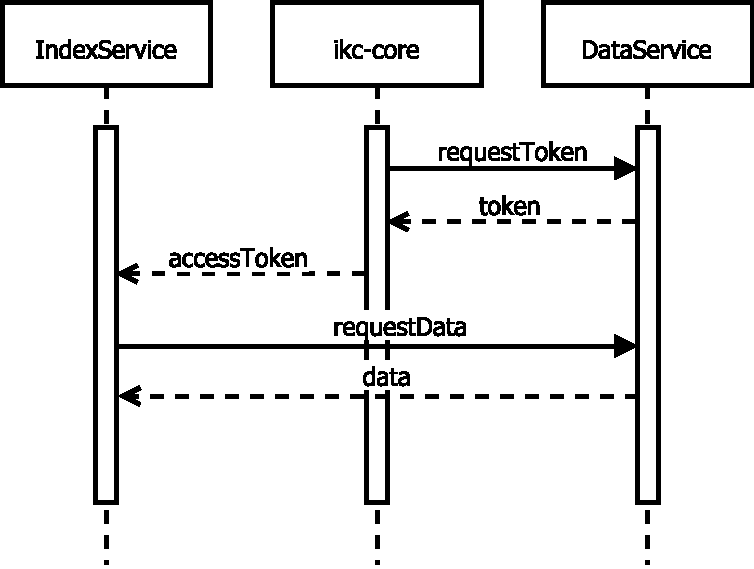
\includegraphics[width=0.8\textwidth]{SeqAccess}
    \caption{Ablauf: Datenfreigabe}
    \label{fig:seqaccesssession}
    \end{figure}
    
    
Nach den obigen Erklärungen zeigt folgender Ausschnitt (\autoref{token-handling}) die Basis der Freigabe-Lösung. Der \texttt{DataService} hält wäh\-rend der Ausführung eine Instanz des Klasse \texttt{Store}. Diese ist unter anderem für die Verwaltung der \gls{Token}[s] zuständig. Auf Zeile 7 ist die Initialisierung einer \texttt{Map} zu sehen. Diese hält zu einem Token (\texttt{string}) einen Zugang (\texttt{AccessSession}). 

Ein Beispielablauf könnte folgendermassen aussehen: Der \gls{ikc-core} will dem \texttt{IndexService} eine Datei freigeben: Vom \texttt{IndexService} trifft eine Anfrage (\texttt{TokenRequest}) beim \texttt{DataService} ein. Darum ruft er die Methode \texttt{addAccessSession} auf. Diese generiert einen \gls{Token} (Zeile 12), hinterlegt diesen in der \texttt{Map}. Schlussendlich wird der \gls{Token} ebenfalls an den \gls{ikc-core} zurückgegeben. Darauf folgt eine Anfrage vom \texttt{IndexService} an den \texttt{DataService}. Nun wird im \texttt{Store} aber die Methode \texttt{getAccessSession} (Zeile 17) aufgerufen. Mittels dem mitgeliefertem \texttt{Token} kann aus der \texttt{Map} des \texttt{Stores} die entsprechende, zuvor abgelegte Berechtigung (\texttt{AccessSession}) abgerufen werden (Zeile 18). Der Zugang wird nach der einmaligen Nutzung gelöscht (Zeile 19). Die \texttt{AccessSession} wird an den \texttt{IndexService} retourniert und er kann damit auf die gewünschten Daten zugreifen.
    
  \begin{listing}[H]
\inputminted[
frame=lines,
framesep=2mm,
baselinestretch=1.2,
linenos,
breaklines=true
]{js}{sourcecode/dataservice/Store.ts}
\caption{Store: Token-Handling}
\label{token-handling}
\end{listing}
  

% ----------------------------------------------------------------

\section{MessageManager}\label{s-message-manager}

% ----------------------------------------------------------------

Sowohl im \texttt{Dataservice} als auch im \texttt{IndexService} wird für die Nachrichtenverarbeitung ein \texttt{Mess\-age\-Man\-ager} verwendet. Ein besonderes Augenmerk liegt dabei auf der Entkopplung der Verarbeitung und der Handhabung der einzelnen Nachrichten. Dazu werden \textit{Traits} verwendet, mit welchen zur Laufzeit das Verhalten einer Klasse angepasst werden kann. Dies geschieht durch die Ersetzung des Verhaltens einer Funktion durch jenes des \textit{Traits}. \autoref{fig:mixin} zeigt die Verwendung von \textit{Traits} innerhalb des \texttt{Mes\-sage\-Man\-agers}.

\begin{itemize}
    \item Die beiden Interfaces \texttt{Mapper} und \texttt{Processor} definieren die beiden Methoden \texttt{send} und \texttt{process}.\\
    \item Innerhalb des \texttt{Processors} wird die Abarbeitung der jeweiligen Nachricht implementiert. Dies geschieht durch die Implementation der \texttt{process} Methode des Interfaces \texttt{Processor}. Dazu wird pro Nachricht eine seperate \texttt{Trait}-Klasse erstellt (zum Beispiel \texttt{DataRequestProcessor} \autoref{data-request-processor}).\\
    \item Die Abbildung des Resultates auf eine Antwort-Nachricht wird durch den jeweiligen \textit{Mapper} (zum Beispiel \texttt{Da\-ta\-Resp\-onse\-Map\-per} \autoref{data-response-mapper}) durchgeführt. Dafür wird die Methode \texttt{map} implementiert, welche durch das Interface \texttt{Mapper} definiert ist.\\    
    \item Als Abstraktion einer eingehenden Nachricht dient die Klasse \textit{Request} (\autoref{message-manager}). Sie enthält die eingegangene Nachricht (\texttt{message}, Zeile 2) und ein \texttt{callback} (Zeile 3), um eine Antwort-Nachricht zurückzugeben. Weiter ist die Methode \texttt{run} (Zeile 7-17) definiert, welche die beiden Methoden \texttt{process} (Zeile 8) und \texttt{map} (Zeile 9) ausführt und die resultierende Antwort-Nachricht zurückgibt (Zeile 10).\\
    \item Innerhalb des \texttt{MessageManagers} wird nun die \texttt{Re\-quest}-Klasse je nach Situation angepasst. Bevor die Eingehende Nachricht mittels der \texttt{run} Methode (Zeile 3) abgearbeitet werden kann, muss das entsprechendes Objekt generiert werden. Dazu wird die Methode \texttt{mixIn} (Zeile 5-12) verwendet, welche je nach Art der Nachricht (Zeile 7) die jeweiligen \textit{Traits} (Zeile 8) zuordnet und ein Objekt der \texttt{Request}-Klasse instanziiert (Zeile 9). Dabei wird die Methode \texttt{applyMixins} (Zeile 14-20) verwendet, welche die beiden Methoden \texttt{process} und \texttt{map} mit den entsprechenden \textit{Traits} überschreibt (Zeile 17).
\end{itemize}

    \begin{figure}[H]
    \centering
    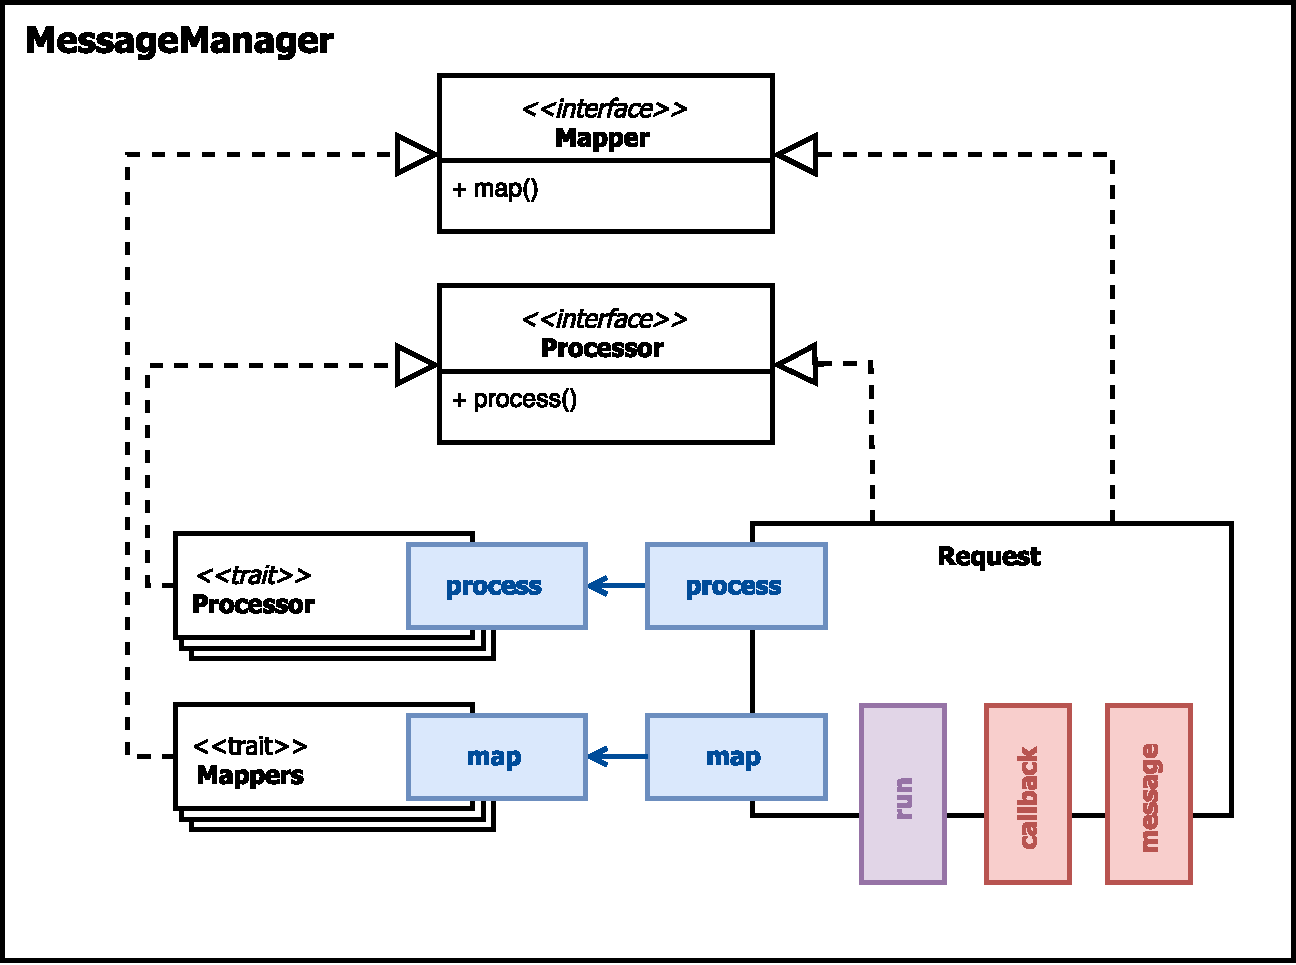
\includegraphics[width=0.8\textwidth]{Mixin}
    \caption{Funktionsweise MessageManager}
    \label{fig:mixin}
    \end{figure}
    
\begin{listing}[H]
\inputminted[
frame=lines,
framesep=2mm,
baselinestretch=1.2,
linenos,
breaklines=true
]{js}{sourcecode/DataRequestProcessor.ts}
\caption{DataRequestProcessor Implementation}
\label{data-request-processor}
\end{listing}

\begin{listing}[H]
\inputminted[
frame=lines,
framesep=2mm,
baselinestretch=1.2,
linenos,
breaklines=true
]{js}{sourcecode/DataResponseMapper.ts}
\caption{DataResponseMapper Implementation}
\label{data-response-mapper}
\end{listing}
    
\begin{listing}[H]
\inputminted[
frame=lines,
framesep=2mm,
baselinestretch=1.2,
linenos,
breaklines=true
]{js}{sourcecode/Request.ts}
\caption{Request-Klasse}
\label{request-class}
\end{listing}


\begin{listing}[H]
\inputminted[
frame=lines,
framesep=2mm,
baselinestretch=1.2,
linenos,
breaklines=true
]{js}{sourcecode/MessageManager.ts}
\caption{MessageManager}
\label{message-manager}
\end{listing}

% ----------------------------------------------------------------

\section{Integration des Prototypen}

% ----------------------------------------------------------------

Der Prototyp soll sich möglichst nahtlos in den \gls{ikc-core} integrieren. Um dies zu erreichen, darf der Prototyp in keiner Situation Funktionen des \gls{ikc-core} blockieren. 

So werden Suchresultate des Indexes innerhalb der bestehenden Suche integriert und bei Bedarf aktualisiert. Die Resultate der verschiedenen Quellen sollen in Echtzeit nach ihrem Eintreffen dargestellt werden. Somit wird sich die Liste der Resultate trotz gleichem Suchbegriff über die Zeit verändern, da weitere Resultate von entfernten Quellen eintreffen. 

Weiter sollen extrahierte \gls{Keyphrase}[s] klar getrennt von den bestehenden Properties des Nodes als \textit{Chips} oberhalb des Titel dargestellt werden. Sowohl ein Dokument mit entsprechenden \gls{Keyphrase}[s] als auch eine \gls{Keyphrase} mit den verknüpften Dokumenten werden als Node dargestellt. \autoref{fig:bda_ui} zeigt einen Entwurf dieser Integration. 

    \begin{figure}[H]
    \centering
    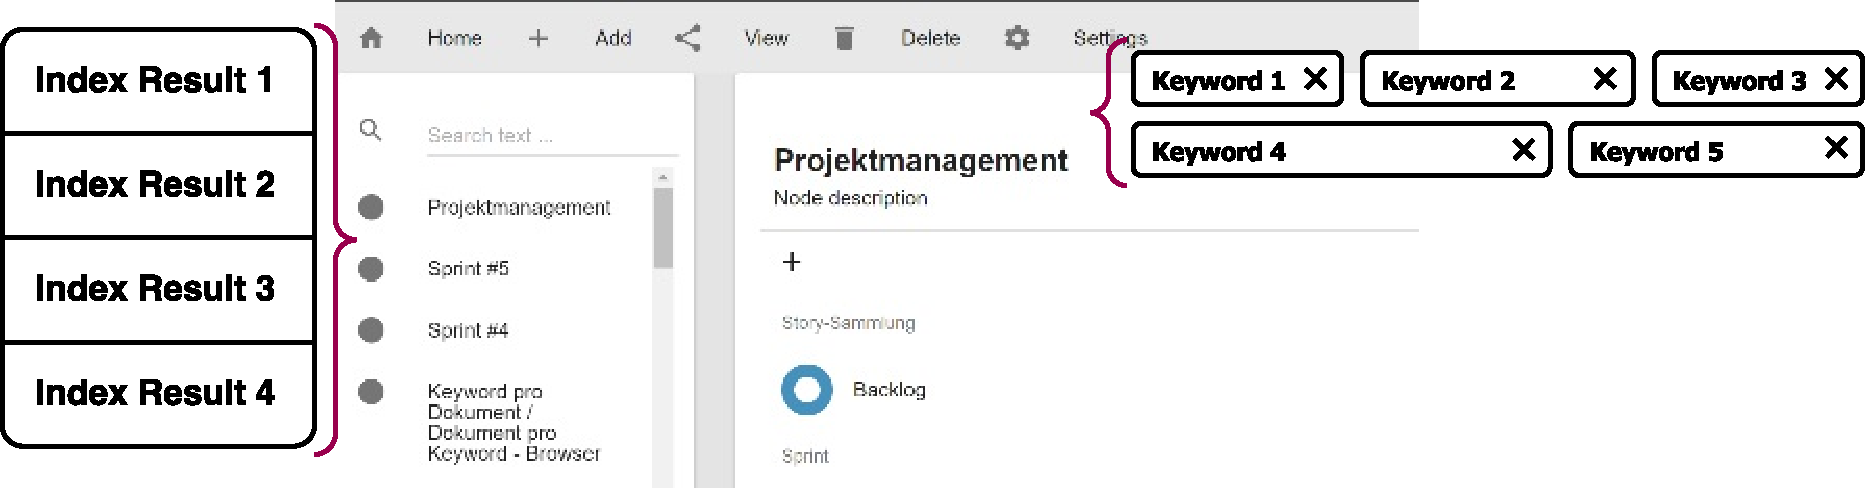
\includegraphics[width=1\textwidth]{BDA_UI}
    \caption{Entwurf Integration Benutzeroberfläche}
    \label{fig:bda_ui}
    \end{figure}

Um die Schnittstellen des Prototyps ideal zu verwenden und die obigen Oberfläche umzusetzen, sind Anpassungen beziehungsweise Erweiterungen in der Software-Struktur des \gls{ikc-core} nötig. Das Klassendiagramm (\autoref{fig:classDiagrammIkcCore}) erläutert die wichtigsten Anpassungen:

\begin{itemize}
    \item Um lokale Suchresultate mit denen des Volltext-Indexes zu kombinieren, wird die \texttt{SearchBroker}-Klasse verwendet. Darin werden Resultate beider Quellen entgegengenommen und für die Darstellung verarbeitet. Mit Hilfe des Interfaces \texttt{SearchResult} und dessen beiden Implementationen \texttt{IndexSearchResult} und \texttt{LocalSearchResult} kann für den jeweiligen Umgang unterschieden werden. Sobald die ersten Suchresultate eintreffen, werden diese verarbeitet und der Benutzeroberfläche weitergegeben. Mit Hilfe der Generalisierung durch das Interface ist es möglich, beliebige Suchquellen in unbegrenzter Anzahl zu integrieren.\\ 
    \item Der \texttt{IndexSearchService} ist verantwortlich für die Kommunikation mit dem \texttt{IndexService} als auch dem \texttt{DataService}. Dazu werden die vorgestellten Protokolle (\autoref{section:protokoll}) verwendet.\\
    \item Um dem Benutzer entfernte Nodes zu präsentieren wird der \texttt{ElementCache} verwendet. Darin werden temporäre Nodes des Indexes (Dokument oder \gls{Keyword}) gespeichert und bei Bedarf für die Benutzeroberfläche bereitgestellt.
    \item Der \texttt{IndexResultProcessor} bildet das Bindeglied zwischen Resultaten des \texttt{IndexService} und dem \texttt{ElementCache}. Er nimmt Resultate des \texttt{IndexService} vom \texttt{IndexSearchService} entgegen, verarbeitet sie und sendet sie weiter an den \texttt{ElementCache}, wo sie anschliessend der Benutzeroberfläche zur Verfügung stehen.\\

\end{itemize}


    \begin{figure}[H]
    \centering
    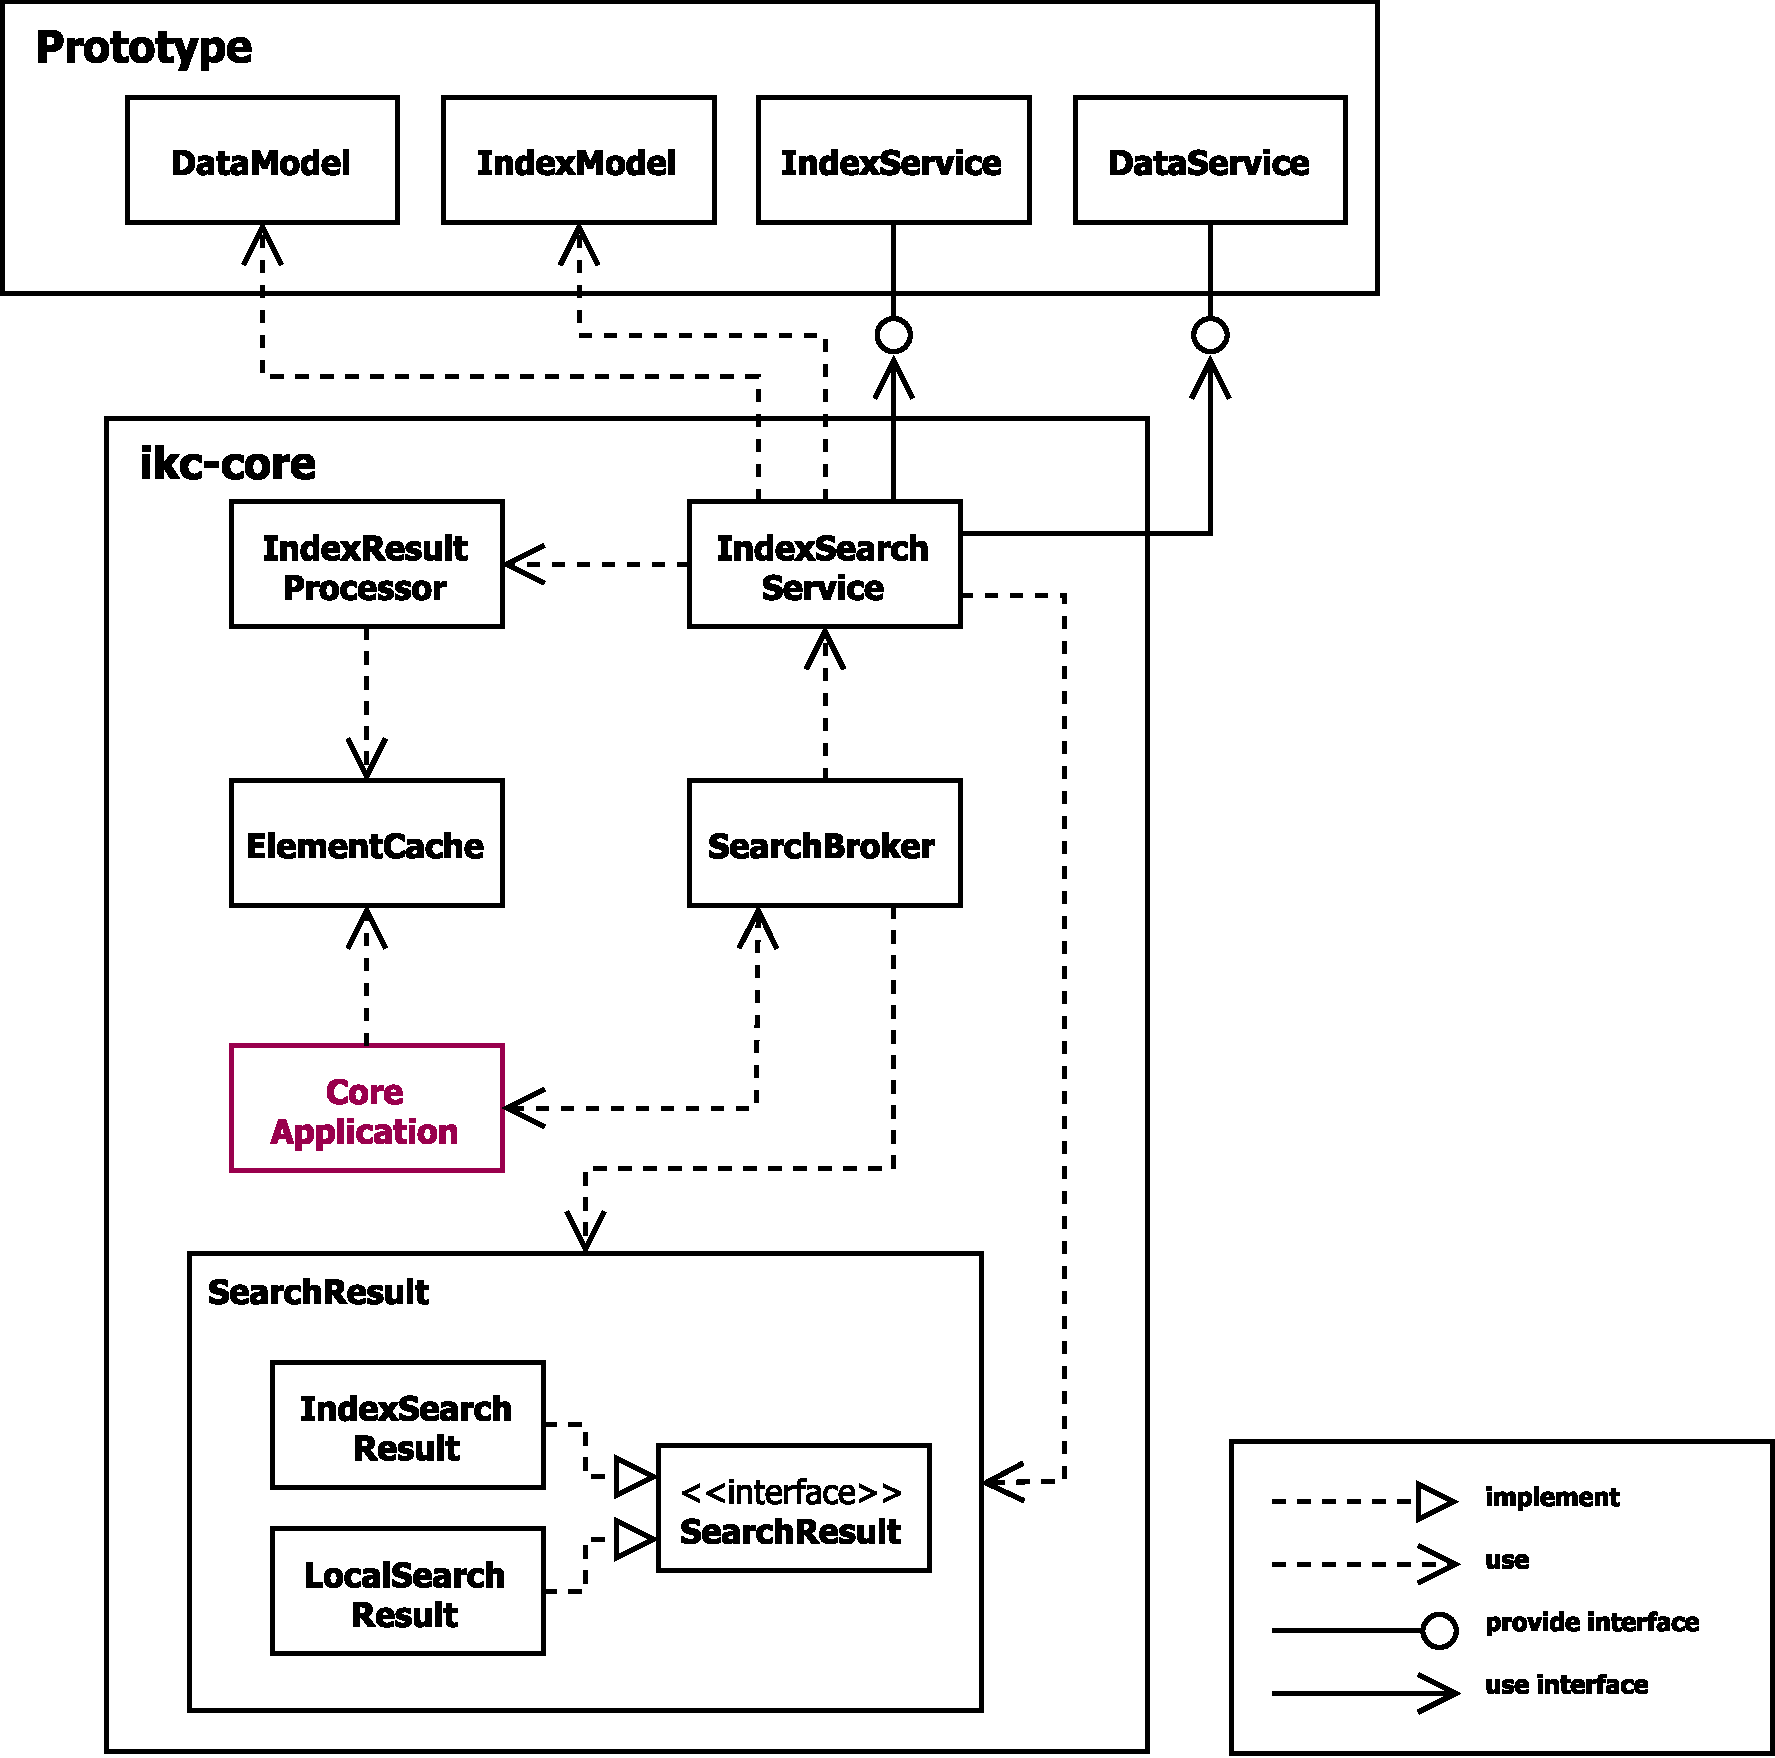
\includegraphics[width=1\textwidth]{ClassDiagrammIkcCore}
    \caption{Klassendiagramm Integration}
    \label{fig:classDiagrammIkcCore}
    \end{figure}
%riesiges index.json, ungefähr 100k Files als Text-Dateien


% ----------------------------------------------------------------

\subsection{Grundsätzliche Anpassung}

% ----------------------------------------------------------------

Insbesondere für die Erweiterung des \gls{ikc-core} mit der Möglichkeit der Kategorisierung von Nodes, mussten einige grundlegende Anpassungen gemacht werden. Die folgenden Zeilen beschreiben diese Änderungen, jedoch werden Kenntnisse des \gls{ikc-core}[s] vorausgesetzt:
\begin{itemize}
    \item Da es neue Arten von Nodes gibt, wurde der Enumerator \verb|NODE_TYPE| mit folgenden Einträge erweitert:
    \begin{itemize}
        \item \verb|INDEX_DOCUMENT|\\
        \item \verb|INDEX_CONCEPT|\\
        \item \verb|DOCUMENT|\\
        \item \verb|CONCEPT|\\
    \end{itemize}
    \item Ebenfalls musste der Enumerator \verb|PROPERTY_TYPE| erweitert werden, um die Verbindung neuer Arten von Nodes verbinden zu ermöglichen:
    \begin{itemize}
        \item \verb|INDEX_DOCUMENT|\\
        \item \verb|INDEX_CONCEPT|\\
        \item \verb|DOCUMENT|\\
        \item \verb|CONCEPT|\\
        \item \verb|BACK_DOCUMENT|\\
        \item \verb|BACK_CONCEPT|\\
        \item \verb|VISIBLE_BACK_DOCUMENT|\\
        \item \verb|VISIBLE_BACK_CONCEPT|\\
    \end{itemize}    
\end{itemize}


% ----------------------------------------------------------------

\subsection{ElementCache}

% ----------------------------------------------------------------

Um Nodes, welche Informationen aus dem externen Index enthalten zu organisieren, wird ein Cache verwendet. Dieser ist innerhalb der Klasse \texttt{ElementCache} implementiert. Darin werden Nodes mit dem Typ \verb|INDEX_DOCUMENT| und \verb|INDEX_CONCEPT| gespeichert. Ein Node durchläuft dabei die folgenden Schritte:
\begin{itemize}
    \item Es werden entweder \gls{Keyphrase}[s] für ein Dokument oder die Dokumente für ein \gls{Keyphrase} bei dem \texttt{IndexService} angefragt. 
    \item Das Resultat wird nun durch den \texttt{Index\-Result\-Pro\-cessor} verarbeitet, in \verb|INDEX_DOCUMENT|- und \verb|INDEX_CONCEPT|-Nodes abgefüllt und im \texttt{ElementCache} gespeichert.
    \item Innerhalb der \texttt{Main}-Komponente des \gls{ikc-core}[s] wird der \texttt{Ele\-ment\-Cache} berücksichtigt, falls der Node im \texttt{NodeModel} nicht gefunden wird (\autoref{main}).
    
    \begin{listing}[H]
    \inputminted[
    frame=lines,
    framesep=2mm,
    baselinestretch=1.2,
    linenos,
    breaklines=true
    ]{js}{sourcecode/Main.ts}
    \caption{Main Komponente}
    \label{main}
    \end{listing}
    
    \item Bei Änderungen an Nodes an einem der Typen \verb|INDEX_DOCUMENT| und \verb|INDEX_CONCEPT|, werden diese in das \texttt{NodeModel} übertragen und aus dem \texttt{ElementCache} gelöscht.

\end{itemize}

% ----------------------------------------------------------------

\subsection{NodeTag}

% ----------------------------------------------------------------
Um dem Benutzer die Möglichkeit zu geben eine Kategorisierung von Nodes vorzunehmen, wurde eine neue \gls{React}-Komponente namens \texttt{NodeTag} erstellt. Sie ist oberhalb des Node-Titels platziert, siehe \autoref{fig:nodetag}, und bietet folgende Funktionalitäten:
\begin{itemize}
    \item Vorhandene Begriffe werden dargestellt, dabei handelt es sich um \texttt{NodeProperties} mit dem Typ \texttt{CONCEPT} oder \verb|INDEX_CONCEPT|.\\
    \item Beliebige Begriffe können als Input definiert werden, diese werden jeweils mit der Tab-Taste bestätigt und hinzugefügt.\\ 
    \item Während der Eingabe neuer Begriffe werden bestehende vorgeschlagen. Die Vorschläge basieren auf der Eingabe. Diese kön\-nen direkt aus der Liste ausgewählt und hinzugefügt werden. (In \autoref{fig:nodetag} Tag4)\\
    \item Bestehende Begriffe können durch einen Klick auf das Kreuz gelöscht werden.\\
\end{itemize}

    \begin{figure}[H]
    \centering
    
\includegraphics[width=1\textwidth]{NodeTag}
    \caption{Integration Kategorisierung}
    \label{fig:nodetag}
    \end{figure}

Für die Bereitstellung von benötigten Informationen und die Abarbeitung von spezifischen Operationen wurden die beiden Klassen \texttt{TagModel} und \texttt{TagService} erstellt. \texttt{TagModel} ist eine Sammlung von bestehenden Begriffen. Diese befüllt die Komponente mit ver\-füg\-bar\-en Vorschlägen anhand einer Liste. Die Aufgabe spezifische Tag-\-Op\-er\-a\-tion\-en durchzuführen erledigt der \texttt{TagService}. Er übernimmt die Aufgabe den entsprechende Tag-Node mit dem geladenen Node zu verknüpfen. Dabei gibt es drei unterschiedliche Szenarien:
\begin{itemize}
    \item Der Tag-Node hat den Type \texttt{CONCEPT} und ist bereits Teil des \texttt{NodeModel}. Somit müssen noch die entsprechenden Ver\-knüpf\-ung\-en erstellt und gespeichert werden.
    \item Der Tag-Node hat den Type \verb|INDEX_CONCEPT| und ist im \texttt{Ele\-ment\-Cache} zwischengespeichert. In diesem Fall muss der Typ des Tag-Node auf \texttt{CONCEPT} geändert werden. Anschliessend wird er im \texttt{NodeModel} gespeichert. 
    \item Der Tag-Node ist weder im \texttt{NodeModel} noch im \texttt{ElementCache} vorhanden und muss komplett neu erstellt werden. Dazu wird ein neuer Node des Typs \texttt{CONCEPT} erstellt, gespeichert und die benötigten Verbindungen erstellt.
\end{itemize}
    

% ----------------------------------------------------------------

\subsection{SearchBroker}

% ----------------------------------------------------------------



% ----------------------------------------------------------------

\subsection{Auto-Indexierung} \label{auto-indexierung}

% ----------------------------------------------------------------

Da SSH Zugriff, ls -a und TimeStamp mit Map vergleichen.

    
% ----------------------------------------------------------------

\section{Deployment}

% ----------------------------------------------------------------


Die \autoref{fig:deployment-diagramm} zeigt das Deployment des \texttt{Prototypen} und des \texttt{Index}- und \texttt{DataServices} auf in den entsprechenden Umgebungen und Services.

    \begin{figure}[H]
    \centering
    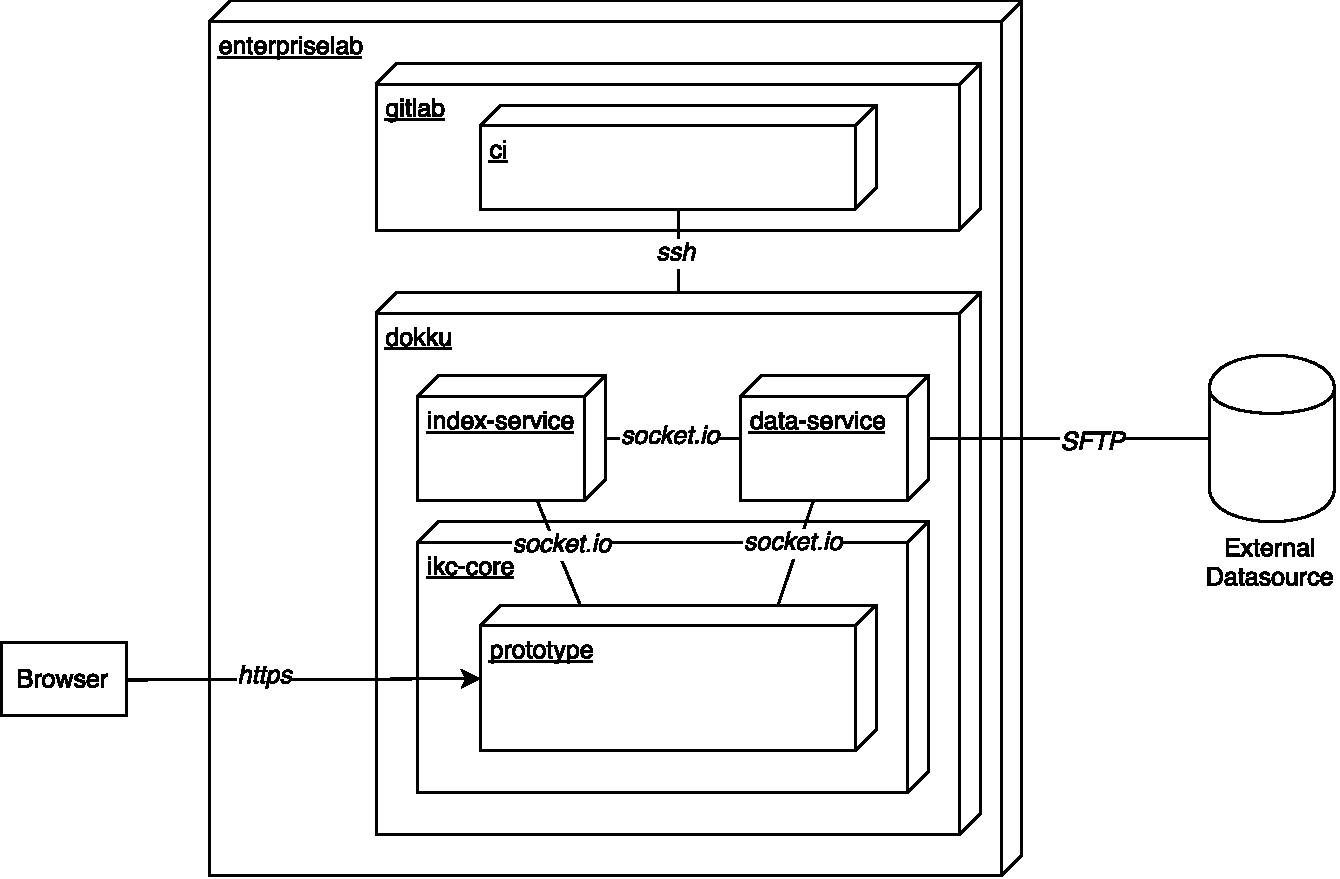
\includegraphics[width=0.8\textwidth]{DeploymentDiagramm}
    \caption{Deployment Diagramm}
    \label{fig:deployment-diagramm}
    \end{figure}

Grundsätzlich liegt jedes Projekt im \gls{gitlab} auf dem vom der Hochschule Luzern zur Verfügung gestelltem \gls{enterpriselab}. \gls{gitlab} ist eine Plattform für Versionskontrolle, Issue-Management, Continuous Integration und -Delivery oder -Deployment. Änderungen an Projekten werden ins \gls{gitlab} geladen, gebuildet und bei Erfolg direkt in eine Entwicklungs- oder Produktionsumgebung ausgeliefert.

Die Basis für die Entwicklungs- beziehungsweise Produktionsumgebungen bildet jeweils ein virtueller \gls{Ubuntu}-Server.
Prinzipiell laufen die Projekte in \gls{Docker}-Container. \gls{Dokku} erleichtert die Handhabung und den Umgang mit dem Netzwerk zusätzlich. Innerhalb vom \gls{Dokku} laufen somit die entwickelten Services wie der \texttt{Index-}, \texttt{DataService} und auch der \texttt{Prototyp}. 

Der \texttt{Prototyp} ist Teil vom bestehenden \gls{ikc-core} und wird clientseitig im Browser ausgeführt. Der \texttt{DataService} nimmt via \gls{SFTP} zusätzlich Gebrauch von einer externen Datenquelle.

% ----------------------------------------------------------------

\section{Benutzerhandbuch}

% ----------------------------------------------------------------


erwähnen und in Anhang
